\documentclass{article}
\usepackage{graphicx}
\usepackage{wrapfig}
\usepackage{subcaption}
\usepackage[margin=1in]{geometry}
\usepackage{amsmath} % or simply amstext
\usepackage{amssymb}
\usepackage{siunitx}
\usepackage{booktabs}
\usepackage[export]{adjustbox}
\newcommand{\angstrom}{\textup{\AA}}
\newcommand{\colormap}{jet}  % colorbar to use
\usepackage{cleveref}
\usepackage{booktabs}
\usepackage{gensymb}
\usepackage{float}
\usepackage{xr}

\externaldocument[S-]{Supporting_Information}

%BJC: potential titles (uncommented is current favorite)
%\title{The Transport Mechanisms of Polar Solutes in a Cross-linked H\textsubscript{II} Phase Lyotropic Liquid Crystal Membrane}
%\title{Size, Shape and Functionality Dependence of Solute Transport Mechanisms in a Cross-linked H\textsubscript{II} Phase Lyotropic Liquid Crystal Membrane}
\title{Chemically Dependent Selectivity in a Cross-linked H\textsubscript{II} Phase Lyotropic Liquid Crystal Membrane}
\author{Benjamin J. Coscia \and Michael R. Shirts} 

\begin{document}

  \graphicspath{{./figures/}}
  \maketitle

  \section{Introduction}

  We need highly selective membranes in order to perform efficient separations.

  H\textsubscript{II} phase lyotropic liquid crystals have densely packed, uniform
  sized pores and have the potential to disrupt conventional membrane separation
  techniques by being selective based not only on size and charge, but on chemical
  functionality as well.

  We can only learn so much from experiment. MD can give us mechanistic insights with
  atomistic resolution so that we can intelligently design new membranes for 
  solute-specific separations.

  In previous work, we determined the most likely structure of the hexagonal phase 
  formed by the monomer Na-GA3C11.
  \begin{itemize}
  	\item We developed techniques for equilibrating the hexagonal phase made by
	neat monomer as well as with varying amounts of water in the pores.
  \end{itemize} 

  In this work, we have studied the transport mechanisms exhibited by a number
  of polar solutes with varying size, chemical functionality and hydrophilic character.
  \begin{itemize}
	\item Many of the separations we are interested in involve polar organic 
	compounds.
  \end{itemize} 

  %BJC1: copied from discussion. Need to work this in the right place
  \begin{itemize}  
  	\item Membranes, including that studied here, are often characterized 
  	with size-exclusion experiments which emphasizes selectivity based on the ability
  	to enter a given pore. 
  	\item Once we reach the nm to sub-nm pore size regime, size-exclusion 
  	becomes of secondary importance since the primary purpose of these membranes is to 
  	separate molecules whose sizes are on the same order as water.
  	\item In order to handle complex waste streams with molecules of similar size,
  	it is important to take advantage of material properties other than pore size. 
  \end{itemize}
  
%  There are a number of questions that we wish to answer in order to create a
%  framework for studying this system in even greater detail.
  \noindent There are a number of questions we wish to address in order to characterize
  transport in this system.
  \begin{enumerate}
  
   	\item What transport mechanisms do we observe? \label{question:mechanisms}
  	
  	Given that the pores will restrict motion of the solutes, we anticipate that 
  	transport will be hindered in some way. We want to understand the differences in
  	solute motion, specifically its mean squared displacement (MSD), based on a solute's
  	size, shape and chemical functionality. We will study the interactions
  	between solutes, the membrane, and water in order to determine which mechanism
  	or mechanisms dominate.
  
  	\item How do molecules, including water, partition within the pores? \label{question:partition}
  	
  	From a macroscopic perspective, it is straightforward to hypothesize that the water and
  	polar solutes spend their time exclusively in the tube-like hydrophilic pore region.
  	Our previous work showed that there is a gradual compositional transition from the 
  	hydrophilic to the hydrophobic region which means that solutes may not 
  	necessarily stay confined to the centers of the pores or even within the
  	pore region. We will study the gradient in composition of solutes and water
  	and any resultant influence it might have on mechanistic properties.
  	
%  	\item Can we describe the transport mechanisms using pre-existing 
%  	mathematical models. \label{question:math}
%  	
%  	A mathematical model may provide additional insight into the transport
%  	mechanisms and, in future work, can help relate performance on the 
%  	timescales studied with MD to macroscopic timescales. We will use
%  	qualitative and semi-quantitative arguments in order to choose a 
%  	governing model. 
  	
  	\item How can we modify the current monomers in order to enhance
  	solute-specific separations? \label{question:math}
  	
  	Most experimental characterization up to this point has been centered 
  	around the monomer, Na-GA3C11, studied here. The primary reason for conducting
  	these simulations is to understand what chemical modifications can be made 
  	to this or similar liquid crystal molecules in order to enhance transport 
  	of desired species or restrict that of undesired species. We will use the 
  	insight gained from our mechanistic observations in order to suggest new 
  	monomer designs.
  	
  \end{enumerate} 
  
  \noindent There are also a number of questions this study is not intended 
  to answer.
  \begin{itemize}
    \item We will not study the concentration dependence of the observed
    transport rates. Although the average MSD might change with concentration,
    we are focused on the underlying solute-membrane interactions that lead to
    the observed transport mechanisms which we conjecture will be the same 
    regardless of concentration.
    \item We will not study the chemical potential of solutes in the pores, which
    could give us a better understanding of equilibrium solute partitioning.
    This information will not greatly enhance our understanding of 
    mechanistic details in various membrane regions.
    \item Both of the above points will add unnecessary levels of complexity
    which can be left for a future study. 
%    \item Our work is meant as a simple starting point for studying transport
%    mechanisms in these complex LLC systems.
    \item This work is a simple starting point meant for observing the types
    of interactions which occur between isolated solutes and the membrane.
  \end{itemize}

  \section{Methods}
  
  Python scripts used to set up systems and conduct post-simulation trajectory 
  analysis are available online at \texttt{https://github.com/shirtsgroup/LLC\_Membranes}.
  The appropriate script to use for each of the following calculations is summarized
  in Table~\ref{S-table:python_scripts} of the SI.
  
  \noindent We ran all molecular dynamics simulations and energy minimizations 
  using GROMACS 2018.3 \cite{bekker_gromacs:_1993,berendsen_gromacs:_1995,van_der_spoel_gromacs:_2005,hess_gromacs_2008} 
  
  \subsection*{System Setup}\label{method:system_setup}

  Stable H\textsubscript{II} phases, assembled with Na-GA3C11, can be formed
  using a broad range of water concentrations.
  \begin{itemize}
	\item In the literature, this system is typically synthesized with close
	to 10 wt \% water \cite{smith_ordered_1997, zhou_new_2007}
    \item However, Resel et al. noted that the system is likely fully 
	hydrated with less than 7 wt \% water. \cite{resel_h2-phase_2000}
	\item We decided to test two different levels of water content: 5 and 10 wt \%
  \end{itemize} 

  %BJC: reference to supporting info with more details on water partition
  %BJC: or should that go in the main body results?
  We observed that water partitions into the tail region of our system and therefore
  built our initial configurations with water in both regions close to the expected
  equilibrium value.
  \begin{itemize}
	\item There is a 2:1 ratio of water in the pores versus in the tails for the 10 wt \% system.
	\item The amount of water present in the tails may or may not be experimentally consistent
	but if we don't put it in, the results will not be thermodynamically consistent, which 
	will give issues with measurements and calculations.
	\item See section~\ref{S-section:water_content_equil} of the SI for further details on 
	water equilibration in this system.
	\item We iteratively adjusted the pore radius in our systems until the right amount of water
	fit in the pores when we ran \texttt{gmx solvate}.
	\item We placed water molecules in the tail region one at a time in random locations
	with short energy minimizations between insertions.
  \end{itemize}

%  We equilibrated the initial configuration using the `wet' equilibration procedure
%  described in our previous work (reference to structure paper).
  %BJC: not sure I need to go into any details describing that procedure
%  \begin{itemize}
%	\item Series of NVT simulations with force constants on carbon atoms of aromatic
%	ring in head group
%	\item Force constants reduced according to the sequence: 1000000, 3162,
%	56, 8, 3, 2, 1, 0 kJ mol$^{-1}$ nm$^{-2}$ 
%  \end{itemize}

%  We cross-linked the equilibrated solvated configuration using the cross-linking procedure
%  described in our previous work. 

  \noindent We equilibrated an initial solvated configuration before adding solutes.
  \begin{itemize}
	\item First, we equilibrated the initial configuration using the `wet'
	equilibration procedure described in our previous work~\cite{coscia_understanding_2019}.
	\item Then we cross-linked the equilibrated solvated configuration using the
	cross-linking procedure described in our previous work.
  \end{itemize}

  \noindent To study a given solute, we added 6 solute molecules to each pore of the
  equilibrated cross-linked configuration.
  \begin{itemize}
	\item We equally spaced each solute in the pore
	\item 6 solutes per pore provided a balance of a useful amount of data
	for generating statistics and a low degree of interaction between solutes (reference
	to supporting information to show low degree of interaction)
	\item At each insertion point we placed a randomly oriented solute molecule
	then ran a short energy minimization.
	\item We allowed the solutes to equilibrate for 5 ns using berendsen 
	pressure control
	\item We collected transport data over the course of 1 $\mu$s MD simulations
  \end{itemize}
  
  \subsection*{Solute Parameterization}\label{method:parameterization}
  
  %BJC: might need to reword. Most of this is taken from my last paper and adapted to solutes.
  Like we have previously done for Na-GA3C11~\cite{coscia_understanding_2019}, we
  parameterized the interaction potential for the solutes using the Generalized 
  AMBER Force Field (GAFF)~\cite{wang_development_2004} with the Antechamber package
  \cite{wang_automatic_2006} provided with AmberTools16~\cite{case_ambertools16_2016}.
  We chose GAFF because it has been parameterized for use with organic molecules. We
  assigned atomic charges using the am1bccsym method of \texttt{molcharge} shipped
  with QUACPAC from Openeye Scientific Software.
  
  \subsection*{Mean Squared Displacement}\label{method:MSD}

  \noindent We measured the time-averaged $z$-direction mean squared 
  displacement (MSD) of the centers of mass of each solute over the 
  course of 1 $\mu$s MD simulations using Equation~\ref{eqn:tamsd}.
  \begin{itemize}
    \item \begin{equation}
	\overline{x^2(\tau)} = \dfrac{1}{T - \tau}\int_{0}^{T - \tau} (x(t + \tau) - x(t))^2 dt
	\label{eqn:tamsd}
	\end{equation}
	where $\tau$ is the time lag and T is the length of the
	trajectory~\cite{meroz_toolbox_2015}. 
	\item Generally, the MSD grows according to Equation~\ref{eqn:msd_form},
	\begin{equation} 
	\langle x^2(t) \rangle = K_{\alpha}t^\alpha
	\label{eqn:msd_form}
	\end{equation} 
	\item where $\alpha$ is the anomalous exponent and $K_\alpha$ is the
	generalized diffusion coefficient.
	\item A value of $\alpha < 1$ indicates a subdiffusive process, while a value of
	$\alpha = 1$ and $\alpha > 1$ is characteristic of Brownian and superdiffusive
	motion respectively.
    % MRS1: time vs. ensemble MSD better in follow-up paper.
	\item In practice, $\alpha$ corresponds to the growth of the \textit{ensemble}
	MSD given by Equation~\ref{eqn:ensemble_msd}~\cite{meroz_toolbox_2015}:
	\begin{equation}
	\langle x^2(t) \rangle = \langle x(t) - x(0) \rangle
	\label{eqn:ensemble_msd}
	\end{equation}
	\item The ensemble MSD is calculated with respect to a reference position and
	hence carries some dependence on its starting point.
	\item The time-averaged MSD averages over all possible time lags of a given 
	length, effectively eliminating any initial configuration dependence and generating
	an increased number of observations. 
	\item For ergodic systems, both types of MSDs will be equal.
	\item Since we have a small number of solutes with which to generate statistics
	and because we are not calculating values for $\alpha$ in this particular study,
	we will only use the time-averaged MSD.
  \end{itemize}  
  
  %BJC: need to word this differently since I haven't talked about CTRW yet
  \noindent We fixed the length of each simulated trajectory so that we could compare
  the total MSD between different solutes without the influence of the ageing phenomenon.
  \begin{itemize}
	\item Ageing is defined by the tendency of the average slope of an MSD curve to decrease
	as the length of trajectories are increased~\cite{metzler_anomalous_2014}.
	\item The maximum measured dwell time can be no longer than the total length
	of a simulated trajectory. 
	\item As measurement time or trajectory length is increased, longer dwell times
	are incorporated into the calculation, lowering the average MSD.
	\item Because the MSDs are non-linear and because of the ageing phenomenon, we
    did not attempt to calculate a diffusion constant as one might for a Brownian
    particle with a linear MSD.
	\item Instead, the reported values for MSD represent the average MSD for a given
	solute after a 400 ns time lag.
  \end{itemize} 
  
%  \noindent Three common mathematical models for modeling anomalous subdiffusion processes include 
%  continuous time random walks (CTRW), fractional Brownian motion (FBM) and
%  random walks on fractals (RWF).\cite{meroz_toolbox_2015}
%  \begin{itemize}
%    \item FBM is common in crowded, viscoelastic environments where each step comes 
%    from a Gaussian distribution but is anti-correlated to its previous 
%    step.~\cite{mandelbrot_fractional_1968,jeon_fractional_2010,banks_anomalous_2005}
%    \item A CTRW is characterized by a distribution of hop lengths and 
%    dwell times, where each each step is characterized by independent random draws from 
%    each distribution.\cite{montroll_random_1965,morrin_three_2018}
%    \item An RWF is imposed by a system's geometry. Systems with tortuous pathways and dead
%    ends cause anti-correlated motion.\cite{meroz_toolbox_2015,neusius_subdiffusion_2008}
%    \item The processes described above can happen alone or in combination.  	
%  \end{itemize}
  
%  \noindent We believe that solutes in the system studied here exhibit subordinated 
%  fractional Brownian motion (sFBM) where the parent process is FBM and the 
%  leading process is a CTRW. 
%  \begin{itemize}
%  	\item The ensemble-averaged MSD differs from the time-averaged MSD, which
%  	is indicative of non-ergodicity, a trait inherent to CTRWs but not FBM or RWFs.~\cite{thiel_weak_2014}
%  	\item We also observe non-stationary $z$-coordinate traces of each solute's
%  	center of mass (COM). %BJC: figure of a z-coordinate trace in main text or in supporting info
%  	\item For a pure CTRW, the time-averaged MSD should be linear.
%  	~\cite{neusius_subdiffusion_2008,meroz_subdiffusion_2010}
%  	\item However, a typical time-averaged solute MSD is sublinear (see supporting
%  	information), which suggests that there is another underlying subdiffusive mechanism.
%  	\item The hop lengths recorded after each dwell period are anti-correlated (See supporting information)
%  	\item Given the viscoelastic nature of the monomers in our system, we believe
%  	the hop lengths can be modeled with FBM. 
% 	\item For subordinated FBM, it can be shown that
%  	\begin{equation}
%  	\langle x^2(t) \rangle \simeq t^{\alpha\beta}
%  	\end{equation}
%  	where $\alpha$ is the anomalous exponent characteristic of the leading CTRW process
%  	and $\beta$ is the anomalous exponent characteristic of the parent FBM process. 
%  \end{itemize}

  \subsection*{Molecular Size Determination}\label{method:molecular_size}
  
  In order to determine an effective radius for each solute, we measured the 
  maximum pairwise distance between atoms of each solute over the course of
  a 2.5 ns simulation of solutes dissolved in a cubic box of water.
  \begin{itemize}
    \item Each box consisted of about 2100 water molecules and 6 solutes.
    \item Although there exist more involved methods for determining the 
    hydrodynamic radius~\cite{schultz_determination_1961}, we chose to use
    a simpler and more intuitive metric since we are only interested in
    observing trends in the solute mean squared displacement as a function
    of solute size. 
  \end{itemize}

%  \subsection*{Dwell and Hop Length Distributions}\label{method:hops_and_dwells}
%
%  %MRS1: we probably only want enough do identify mechanism not to fit anything.  Think about minimum needed for physical understanding.
%  %BJC1: right, the following is the bear minimum if we want to mention dwell time and hop lengths at all. Otherwise this can be omitted.
%
%  \noindent We measured the distribution of dwell times and hop lengths in order to test
%  the hypothesis that solutes follow a CTRW process.
%  \begin{itemize}
%	\item We used the \texttt{ruptures} python package in order to identify
%	breakpoints, times when hops occur, in solute trajectories.\cite{truong_ruptures:_2018}
%%	(See Supporting Information for more details on chosen parameters. i.e. type of cost 
%%	function, cost function penalty	tolerance, number of dimensions used)
%	\item The corresponding hop lengths and dwell times between break points were 
%	used to construct empirical distributions.
%  \end{itemize}
  
  \subsection*{The Stokes-Einstein Relationship}\label{method:stokes}
  
  The Stokes-Einstein relationship expresses the diffusion coefficient of 
  a hard spherical particle as a function that is inversely related to the
  particle's radius:
  \begin{itemize}
  	\item $D = \dfrac{k_bT}{6\pi\eta r}$
  	\item where $k_b$ and $T$ are the Boltzmann	constant and the system 
  	temperature respectively and $\eta$ is the system's viscosity.
  	\item For the largely demonstrative calculations relevant to this study, 
  	we assume that the system viscosity is constant since we only make minor
  	changes to the membrane's composition and accurately assessing the viscosity
  	in a complex and inhomogeneous system such as ours is a challenge by itself.
  	\item Additionally, rather than calculate $D$, we will apply the relationship
  	to analyze solute MSDs, which is valid because all trajectories are of the same
  	length.
  \end{itemize}
  
  \noindent It is well-known that the relationship breaks down when solute size becomes
  on the order of solvent size because the solute can no longer be treated
  as a non-interacting hard sphere. % citation
  \begin{itemize}
    \item Gierer and Wirtz introduced a microfriction correction factor in order to 
    address this issue. 
    \item They proposed that $D = \dfrac{k_bT}{6\pi\eta fr}$
    %\item Where $f = \left(1.5\dfrac{r_2}{r_1} + \dfrac{1}{1 + \dfrac{r_2}{r_1}}\right)^{-1}$
    \item Where $f = \left(1.5(r_2/r_1) + \dfrac{1}{1 + (r_2/r_1)}\right)^{-1}$
    \item and $r_1$ and $r_2$ are the radii of the solute and solvent molecules
    respectively.
  \end{itemize}

  \subsection*{Radial Density Functions}\label{method:rdfs}
  % BJC1: Should it be Radial Distribution Functions?

  We measured the average radial distance of each solute of interest from the pore
  centers.
  \begin{itemize}
	\item We binned the radial distances and then normalized by the volume
	of the annulus defined by the bin edges.
	\item Although the pores are often described as straight, they have a
	small degree of tortuosity which disrupts the RDF calcuation.
    % MRS1: can you report numerically the tortuosity?
    % BJC1: added at end of paragraph after introduction of splines since tortuosity calculation uses splines.
	\item We tried to mitigate the effects of tortuosity by calculating the RDF
	with respect to splines that run through the pore centers.
%    \item We construct the splines by dividing the membrane into 10 slices
%	in the $z$-direction. Within each slice, we calculate the location of 
%	the pore centers based on the average location of the aromatic rings
%	that make up the monomer head groups.
	\item Each spline consists of 10 points, equally spaced in the $z$-direction, whose
    ($x$, $y$) coordinates are defined based on the center of mass of all head
    groups closest, in $z$, to the given point.
	\item When calculating RDFs, the radial distance from the pore center
	is based on the distance between the solute center-of-mass and the linearly
	interpolated ($x$, $y$)	coordinates of the pore center calculated based
	on the spline.
	\item Using the splines, we calculated the tortuosity of the 
	pores by calculating the ratio $\dfrac{L}{Z}$ where $L$ is the length of the spline and $Z$ is 
    the length of the unit cell in the $z$-direction. 
    \item The average tortuosity of each pore is 1.03 $\pm$ 0.01 and 1.07 $\pm$ 0.02 in the 
    5 and 10 wt \% systems respectively. 
%    \item Although the value of tortuosity is low, the author's experience suggests
%    that a spline is still justified.	
  \end{itemize}
  
  \subsection*{Identification of Hydrogen Bonds}\label{method:hbonds}

  %MRS1: We want to be able to say that conclusions are independent of reasonable changes in the definition so
  %we are not picking and choosing results (either consciously or unconsciously) 
  Based on the geometric criteria proposed by Luzar and Chandler \cite{luzar_effect_1996},
  we determined a hydrogen bond to exist if the distance between the donor, D, and acceptor,
  A, atoms is less than 3.5 \AA~and the angle formed by D--H...A is less than 30\degree.
    %BJC: According to Luzar/Chandler: The range of a water molecule’s first coordination
    % shell is 3.5 Å, as determined from the oxygen-oxygen radial distribution function.
    % The amplitude of librations that break hydrogen bonds is ,~ 30 degrees, as estimated
    % from Debye-Waller factors
  \begin{itemize}
    \item Attempts to describe a hydrogen bond in the context of molecular simulations has
    yielded a number of definitions with no true consensus \cite{prada-gracia_quest_2013}.
	\item The geometry of hydrogen bonds has some dependence on the system being studied. 
    \item The definition of Luzar and Chandler is easily visualized for trajectories using
    the \texttt{hbonds} representation of the Visual Molecular Dynamics (VMD) software 
    package which allows us to directly check the validity of identified hydrogen bonds.
    \item In section~\ref{S-section:hbond_sensitivity} of the SI, we show that our 
    conclusions are insensitive to this definition within a reasonable range.
    %BJC: might need to update this if something better exists for nitrogen 
  \end{itemize}

  \subsection*{Coordination number}\label{method:coordination}

  We quantified the coordination of solute constituent atoms with sodium ions.
  \begin{itemize}
  	\item For each frame, we counted the number of coordinated molecules to a
  	given solute atom based on a distance cut-off. 
  	\item Using four different methods, Rowley and Roux observed peaks in the
  	radial distribution function for sodium coordinated with water at an O-Na
  	distance of between 2.3 and 2.5 \AA~\cite{rowley_solvation_2012}. 
  	\item We used 2.5 \AA~as the distance cutoff.
  	\item We found that this approach is more useful than calculating the
	3D spherical radial distribution function because it gives detailed
	frame-by-frame information rather than an average. 
  \end{itemize}
  
  Using our procedure we found that sodium ions in a solution of tip3p water
  coordinate with an average of 3.4 water molecules.
  \begin{itemize}
    \item We created a 4 x 4 x 4 nm cubic box of water with the GROMACS tool,
    \texttt{gmx solvate}
    \item We used \texttt{gmx genion} to replace water molecules with sodium
    and chloride ions in order to create a 0.6 M NaCl solution.
    \item We let the system simulate for 5 ns and reported the average
    number of coordinated water molecules per frame after discarding the first ns of 
    simulation. % need to actually do this
    \item We found that the reported average value is not sensitive to NaCl
    concentration (See section~\ref{S-section:coord_number} of the SI)
  \end{itemize}
   
  \section{Results and Discussion}
  
  \subsection*{Structure of Membrane Constituents}\label{section:membrane_components}
  
  Before beginning the analysis of transport behavior, it is important to elucidate
  the topology of the membrane pores.  
  
  %BJC: Do analysis on pure water system for this section.  
  
  In contrast to our previous work with a solvent-free version of this membrane, the pore
  region of the 5 and 10 wt \% water systems are primarily filled with water and sodium
  ions.
  \begin{itemize}
    \item In dry systems, the pore center is densely filled with sodium ions and 
    head groups (See Ref~\cite{coscia_understanding_2019}).
    \item Figure~\ref{fig:component_densities} plots the densities of each
    membrane constituent in the 5 and 10 wt \% systems.
    \item Water is densest at the center of each pore. 
    \item Sodium ions are densest between the pore center and the peak head group density (black dashed line).
    \item The peak density of sodium ions is not at the pore center in either case
    likely because they are still loosely associated with the monomer's 
    carboxylate head groups.
  \end{itemize}
  
  \noindent Pores in the 10 wt\% water system are wider and less crowded by monomers than
  those in the 5 wt\% water system.
  \begin{itemize}
    \item The peak head group density of 10 wt\% water systems is about 0.2 nm
    further from the pore center than the 5 wt\%
    \item The 5 wt \% water system has a non-negligible amount of tail group atoms
    that occupy the pore center.
    \item Based on these observations, we expect solute transport to be fastest 
    in the 10 wt \% system.
  \end{itemize}
  
  % BJC1: Should I show a dry system?
  \begin{figure}[!htb]
  \centering
  \begin{subfigure}{0.415\textwidth}
  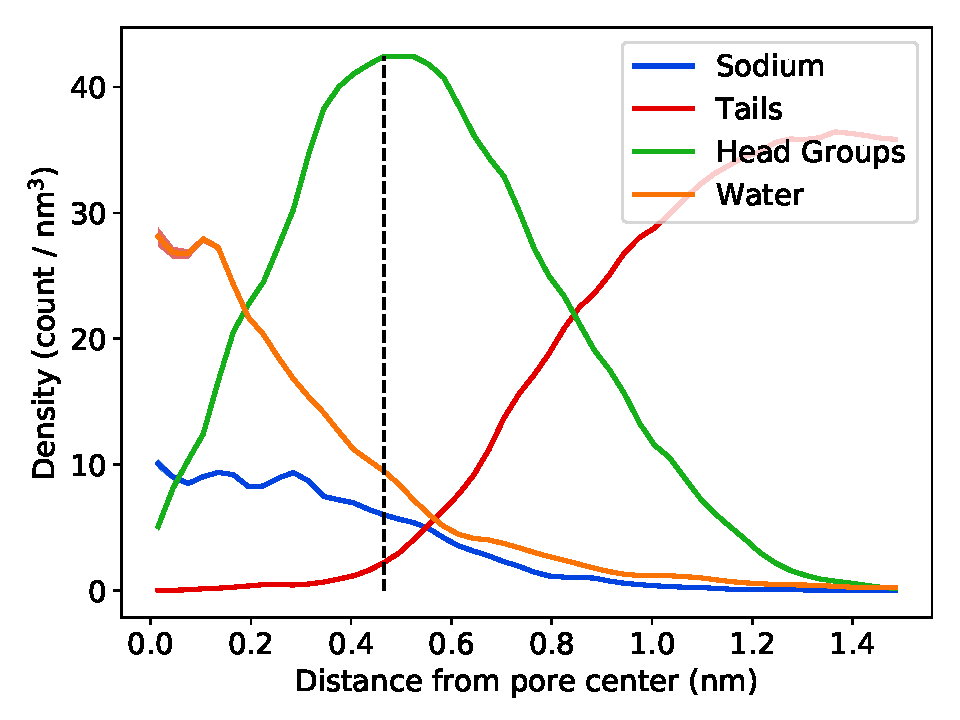
\includegraphics[width=\textwidth]{component_density_5wt.pdf}
  \caption{5 wt\% water}\label{fig:component_density_5wt}
  \end{subfigure}
  \begin{subfigure}{0.15\textwidth}
  \vspace{-0.5cm}
  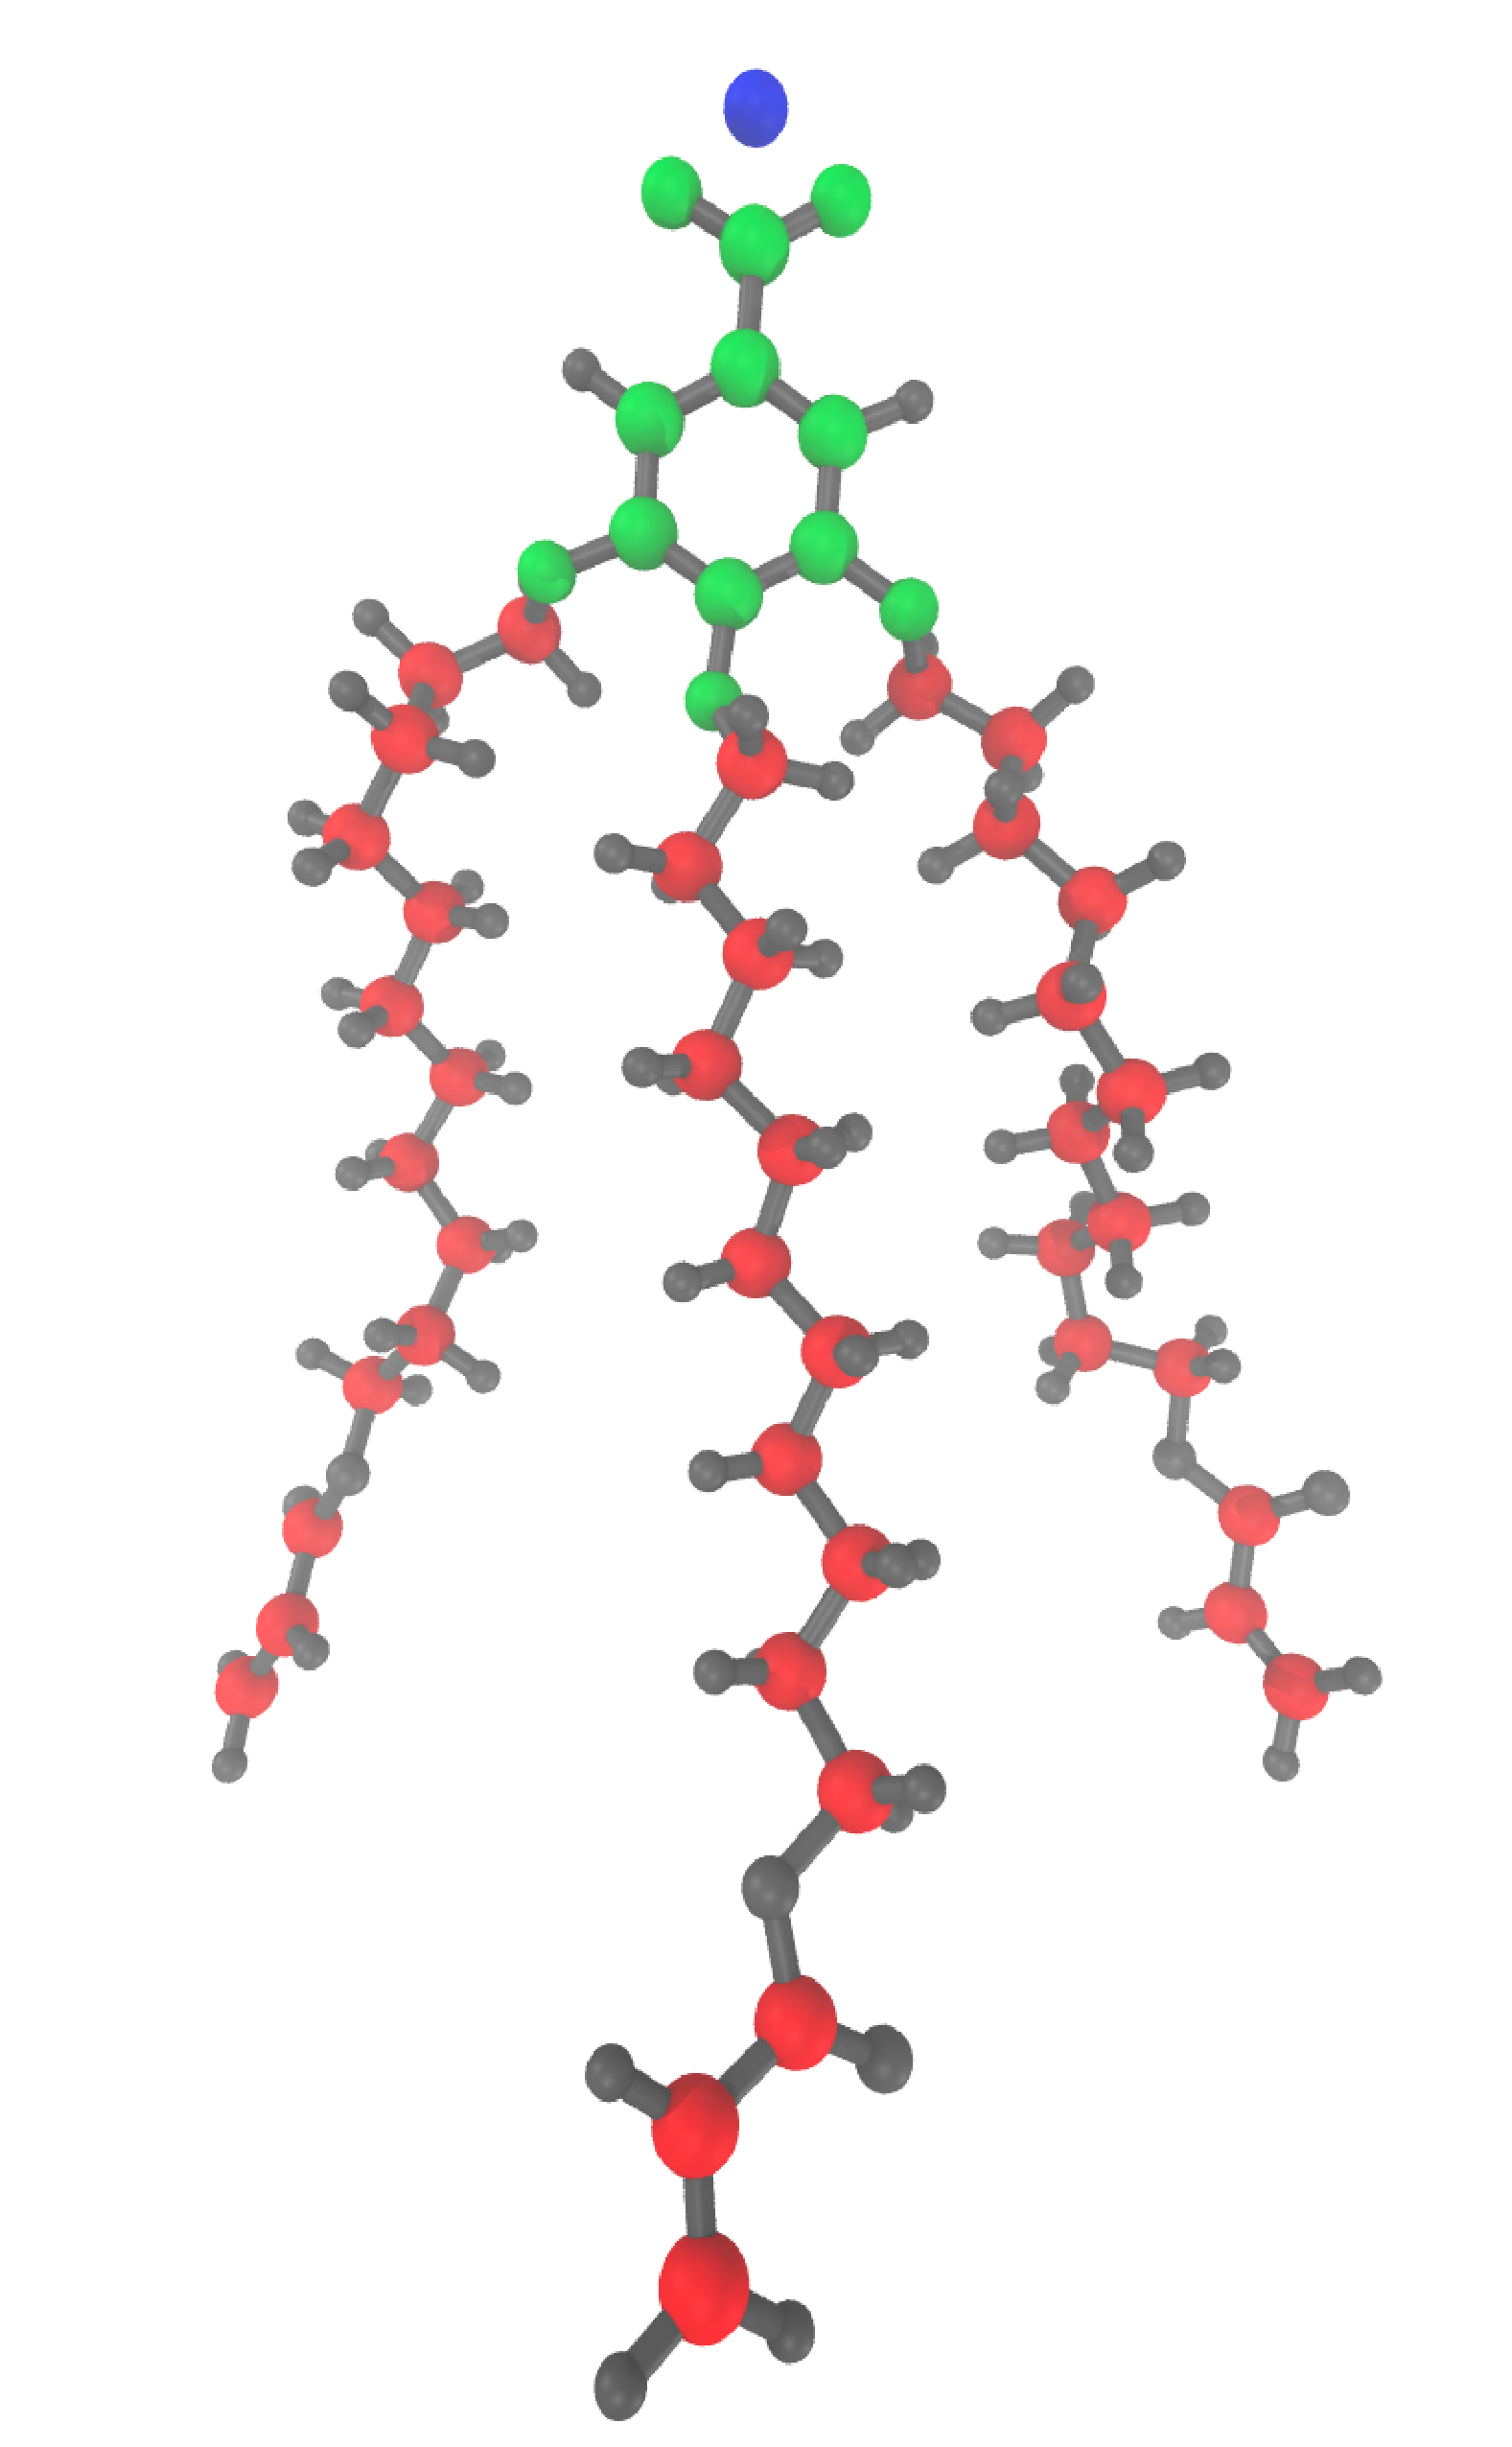
\includegraphics[width=\textwidth]{monomer_color_coded.pdf}
  \label{fig:monomer_color_coded}
  \end{subfigure}
  \begin{subfigure}{0.415\textwidth}
  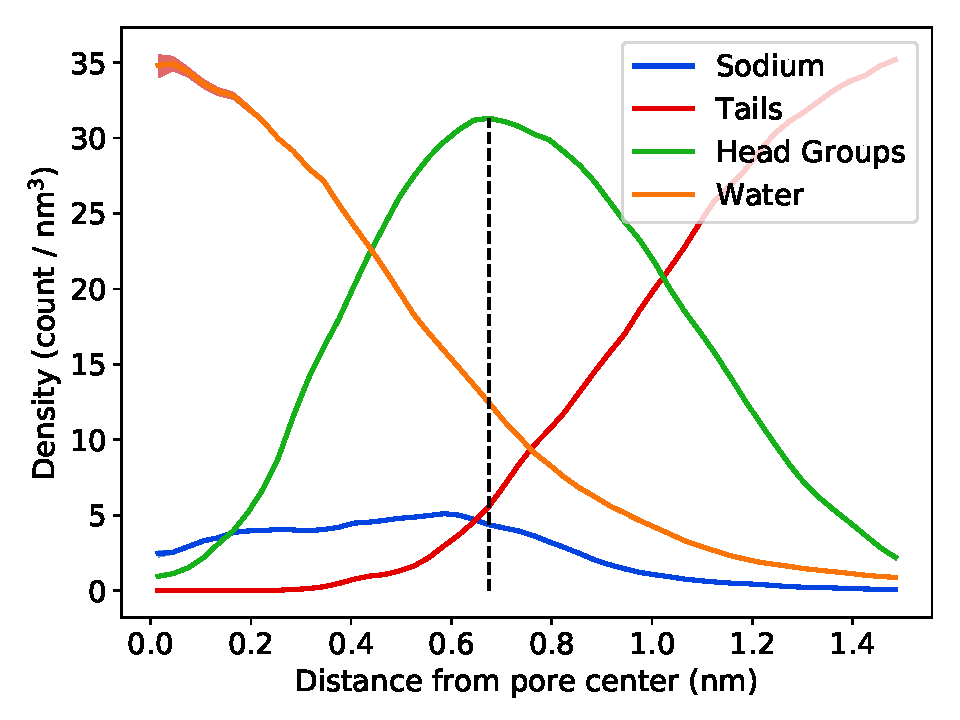
\includegraphics[width=\textwidth]{component_density_10wt.pdf}
  \caption{10 wt\% water}\label{fig:component_density_10wt}
  \end{subfigure}

  %MRS1: possibly include vertical dotted line to show where max head group peak occurs.
  %BJC1: tried it out. Seems like a good addition.
  \caption{The radial densities of various monomer components paint a picture of the
  pore topology where the pore centers are primarily composed of water and sodium ions.
  All RDFs represent the number of atoms located at a given distance from the pore center
  normalized by the volume of the annular bin to which they belong. The pores of the 5 
  wt \% system (a) appears to be much more crowded by monomers than the 10 wt \% system (b).
  Head groups in (a) are densest about 0.2 nm closer to the pore center than in (b). 
  A small amount of tail components find their way close to the pore center of the 5 wt \% system.
  }\label{fig:component_densities}
  \end{figure}

  \subsection*{Mechanisms Governing Small Solute Transport}\label{section:mechanism_overview}

  We observed transport of sodium, water and 20 other small polar solutes inside the
  membrane nanopores. 
  \begin{itemize}
  	\item First, we will comment on transport of the membrane constituents, water and sodium,
  	in a system absent of any additional solutes.
%    \item There are significantly more water molecules and sodium ions in the membrane
%    than solutes.
    \item Then we will present the general trends that we observe among the set of 
    solutes studied.
  \end{itemize}
  
  \subsubsection*{Water and Sodium Ions}\label{section:transport_water_sodium}

%  The MSD of sodium and water is significantly larger in the 10 wt \% water system
%  versus the 5 wt \% water system.
  \noindent Water's mobility is increased when pores are larger and less crowded.
  \begin{itemize}
    %BJC: these numbers will change. This is for incomplete methanol systems. I will
    % redo calculations on pure water systems.
    \item The MSD of water is about 65 times higher and the MSD of sodium is about 40
    times higher in the 10 wt\% system.
    \item Water moves about 65 times faster than sodium in the 10 wt \% system and
    40 times faster than sodium in the 5 wt \% system. %BJC: weird coincidence
    \item The diffusivity of water in the 10 wt \% system is still only 1 \% that of 
    bulk water %BJC: 5.53e-07 versus 5.5e-05 cm^2/s
  \end{itemize}
  
  % BJC: could talk about subdiffusion a little here but I'd rather save it for 
  % small molecule discussion
  
%  \noindent The diffusion constant of water is about 50 times faster than sodium.
%  \begin{itemize}
%    \item In a dilute sodium chloride solution, the diffusivity of sodium
%    is about 4 times slower than water.
%    \item The carboxylate groups, whose oxygen atoms each have a charge of -0.822
%    keep the positively charged sodium ions relatively close and restricts their
%    motion.
%  \end{itemize}
  
  \begin{figure}[!htb]
  \centering
  \begin{subfigure}{0.45\textwidth}
  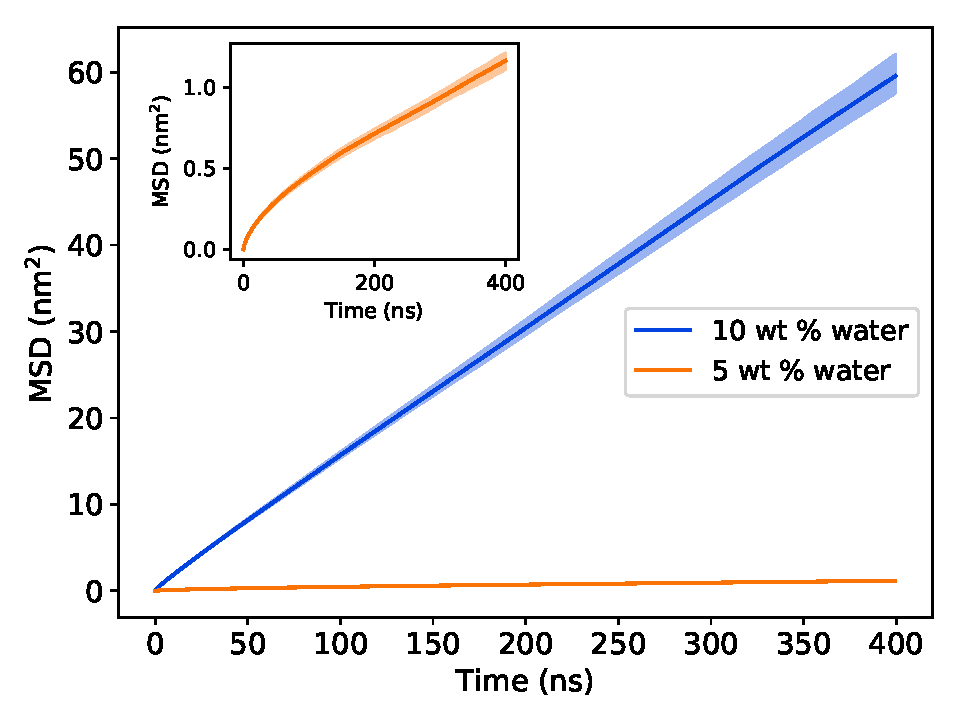
\includegraphics[width=\textwidth]{water_msd_comparison.pdf}
  \caption{Water}\label{fig:water_msd_comparison}
  \end{subfigure}
  \begin{subfigure}{0.45\textwidth}
  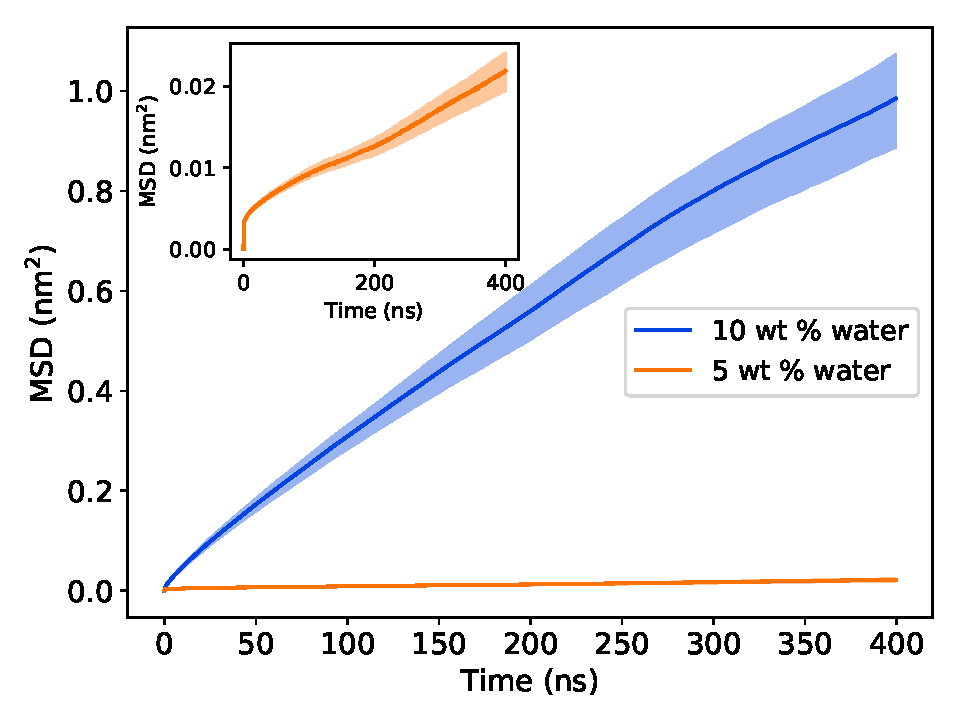
\includegraphics[width=\textwidth]{na_msd_comparison.pdf}
  \caption{Sodium Ions}\label{fig:na_msd_comparison}
  \end{subfigure}
  \caption{(a) The MSD of water in the 10 wt \% water system is about 65 times
  higher than water in the 5 wt \% water system. (b) The MSD of sodium in the
  10 wt \% water system is about 40 times higher than sodium in the 5 wt \% 
  water system.}\label{fig:msd_comparison}
  \end{figure}
  
  \noindent Sodium coordinates with far less water molecules than it does in 
  bulk solution.
  \begin{itemize}
    \item Compared to 3.4 coordinated water molecules in bulk solution (see 
    section~\ref{method:coordination}), sodium ions in our system are, on average,
    coordinated to about 1.7 water molecules in the 10 wt \% system and 1.2 water
    molecules in the 5 wt\% system.
    \item The low levels of water coordination under confinement are likely driven
    in part by favorable interactions between sodium ions and carboxylate head groups.
    \item A dehydrated sodium ion is not well shielded from the negatively charged 
    carboxylate group.~\cite{ma_drastically_2019}. 
    \item On average, sodium ions coordinate with 0.5 carboxylate group oxygen atoms in the
    10 wt \% water system and 0.4 carboxylate oxygen atoms in the 5 wt \% water system. 
    % BJC: I thought 5 wt \% might be a little higher. These numbers might be skewed by
    % sodium ions that are within cutoff of both carboxylate oxygen atoms. Might be
    % better to report average number of sodiums coordinated to a head group
  \end{itemize}
  
  % BJC: This figure is from methanol simulations. Will be replaced by pure water
  % simulations
  % BJC: I can probably just report the averages rather than plot this
  %MRS1: yeah, this is not really worth a graphic.
%  \begin{figure}[!htb]
%  \centering
%  \begin{subfigure}{0.45\textwidth}
%  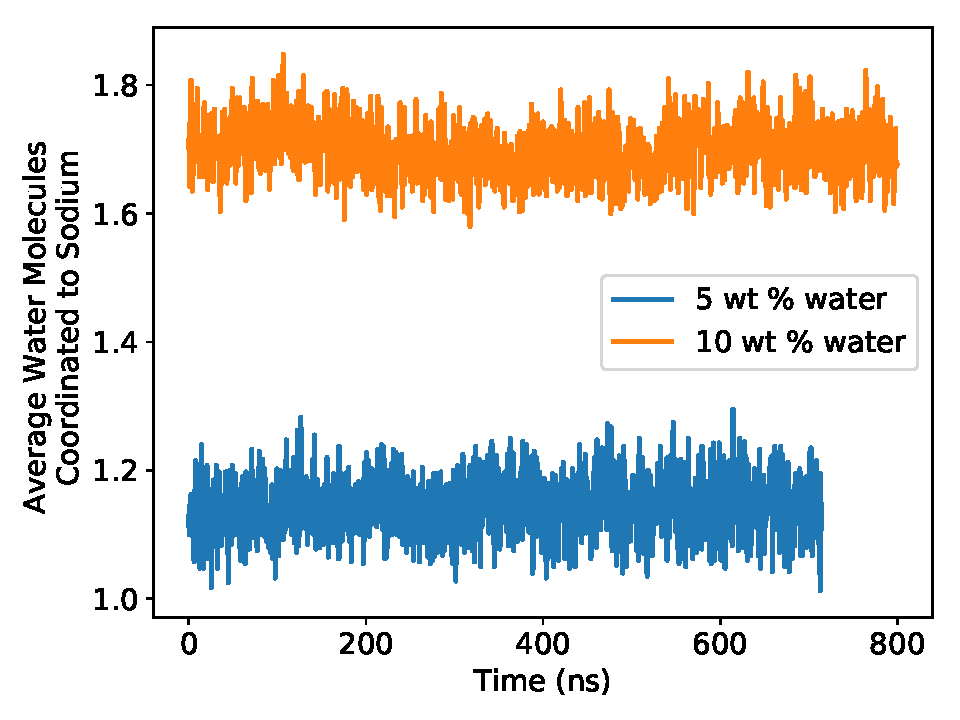
\includegraphics[width=\textwidth]{Na_water_coordination.pdf}
%  \caption{}\label{fig:na_water_coordination}
%  \end{subfigure}
%  \begin{subfigure}{0.45\textwidth}
%  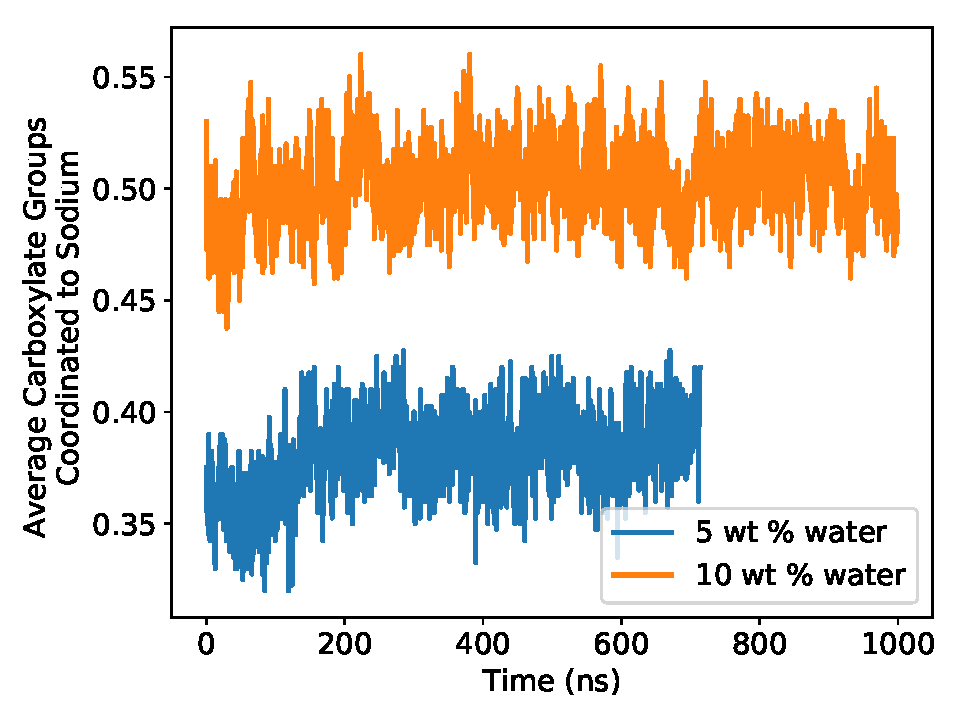
\includegraphics[width=\textwidth]{Na_hg_coordination.pdf}
%  \caption{}\label{fig:na_hg_coordination}  % No caption since this probably won't be a figure
%  \end{subfigure}
%  \end{figure}
  
  \subsubsection*{Transport of Small Polar Solutes}\label{section:general_transport_solutes}  
  
  We observe trends in transport properties that are dependent on chemical 
  environment within the nanopores as well as the chemical functionality of membrane
  constituents rather than just solute size. 
  \begin{itemize}
    \item Polar solutes are slowed by interactions between monomer functional groups
    and ions.
    \item Solutes with hydrophobic character partition out of the pore and are 
    slowed by densely packed organic monomer components.
    \item A thorough understanding of these interactions will help us to create
    monomer design principles.
    \item We will begin our analysis by considering the collective trends observed  
    across all systems and then focus on subsets of similar molecules where 
    some exceptions occur. 
  \end{itemize}
  
%  We have gained a clearer picture of the general transport properties exhibited by
%  this system through the collective study of all solutes. We will first address the
%  questions posed in the introduction in a general sense before addressing them with
%  respect to specific molecules, where exceptions occur.
%  \bigskip
  
  Like water and sodium above, the MSDs of the solutes studied in this work are 
  significantly larger in the 10 wt \% system, than those in the 5 wt \% water 
  system (Figure~\ref{fig:msds}). 
  \begin{itemize}
    \item The fastest moving solute in both cases, methanol, has an MSD about 175
    times larger in the 10 wt \% versus the 5 wt \% system.
    \item Clearly the equilibrium water content of a given LLC system will 
    determine its viability for real separations.
  \end{itemize} 
  
%  \noindent The MSDs for the solutes studied in this work span a moderate range. 
%  \begin{itemize}
%    \item We plotted the 400 ns time-lag MSD for each solute in Figure~\ref{fig:all_msds}.
%  	\item The fastest solute, methanol, has an MSD over 20 times greater than
%  	the slowest, dimethyl formamide. 
%  \end{itemize}
  
  \noindent The MSDs depend on more than just solute size.
  \begin{itemize}
  	\item We plotted the solute size against their MSDs in Figure~\ref{fig:msd_radius_5wt}
  	and~\ref{fig:msd_radius_10wt}.
%  	\item Based on the Stokes-Einstein relationship, it is expected that
%  	the solute MSDs should be inversely related to solute size.
%  	\item Once solute and solvent are of comparable size, the relationship breaks
%  	down and tends to underestimate the MSD. 
%  	\item Gierer and Wirtz introduced a microfriction factor as theoretical
%  	correction.
%  	\item It is expected that the Stokes-Einstein relationship, which assumes that 
%  	the solute radius is much larger than the solvent, should break down once
%  	solute and solvent are of comparable size.
  	\item Assuming that the Stokes-Einstein relationship is no longer valid 
  	for solutes with a radius less than x nm, we fit the Stokes-Einstein relationship 
  	with and without the correction factor making sure that the two curves intersected
  	at x nm and that the corrected line passed through the highest MSD data point, methanol. %BJC1: need a justified value for x. Can also show its insensitivity to choice of intersection point.
  	\item We believe methanol is subject to the least hindrance due its small
  	size and relatively fast motion.
  	\item Although both curves are approximations, they illustrate that
  	the majority of solutes in our study show lower than expected MSDs. 
  	\item In most cases, the predicted MSDs even fall below the 
  	conservative Stokes-Einstein estimate.
  	\item It is clear that more complex mechanisms determine the MSDs of
  	these solutes.
%  	\item There are numerous examples of solutes in our study that do not 
%  	follow the behavior set forth by the Stokes-Einstein equation which 
%  	implies that solute MSD should be inversely related to solute size.  % citation
%    % MRS1: can you plot on the figure what the relatioship SHOULD look like?  It sort of looks linear-ish (especially 5).
%  	\item This behavior is not entirely surprising but worth emphasizing. 
	%BJC1: below moved to intro
%  	\item Membranes, including that studied here, are often characterized 
%  	with size-exclusion experiments which emphasizes selectivity based on the ability
%  	to enter a given pore. 
%  	\item Once we reach the nm to sub-nm pore size regime, size-exclusion 
%  	becomes of secondary importance since the primary purpose of these membranes is to 
%  	separate molecules whose sizes are on the same order as water.
%  	\item In order to handle complex waste streams with molecules of similar size,
%  	it is important to take advantage of material properties other than pore size. 
%  	\item Tetrose, our fifth largest solute, has an average MSD higher than more 
%  	than half of all solutes studied. 
%  	\item The two slowest solutes, DMF and THF, are smaller than 10 faster solutes.
%  	\item Transport is clearly affected by factors other than molecular size. 
  \end{itemize}
  
  \begin{figure}
  \centering
  \begin{subfigure}{0.45\textwidth}
  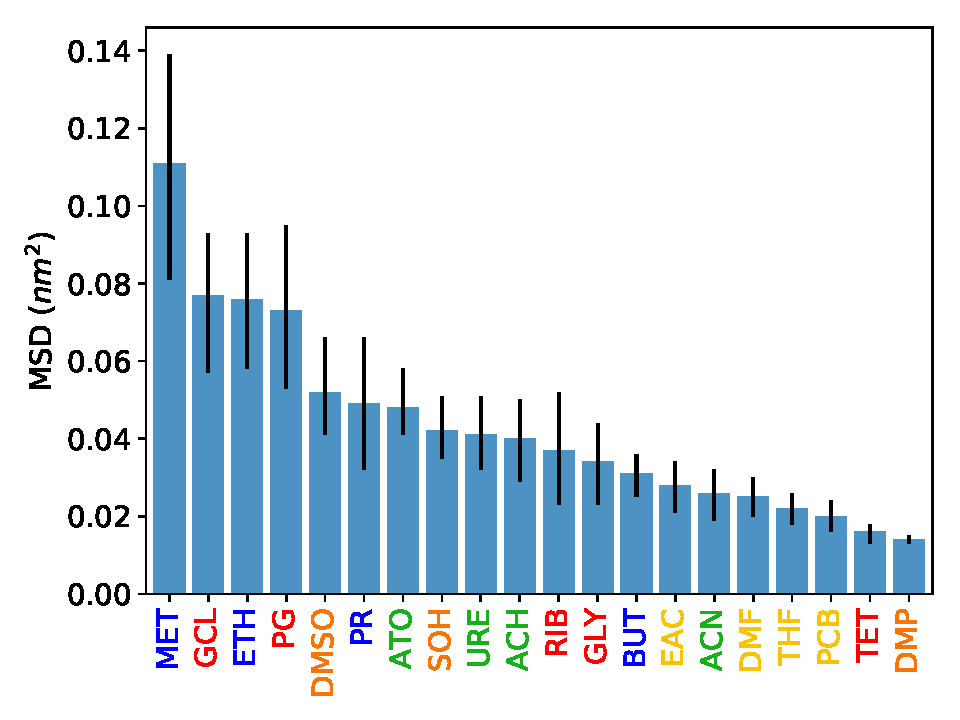
\includegraphics[width=\textwidth]{all_5wt_tamsds.pdf}
  \caption{5 wt \% water}\label{fig:all_msds_5wt}
  \end{subfigure}
  \begin{subfigure}{0.45\textwidth}
  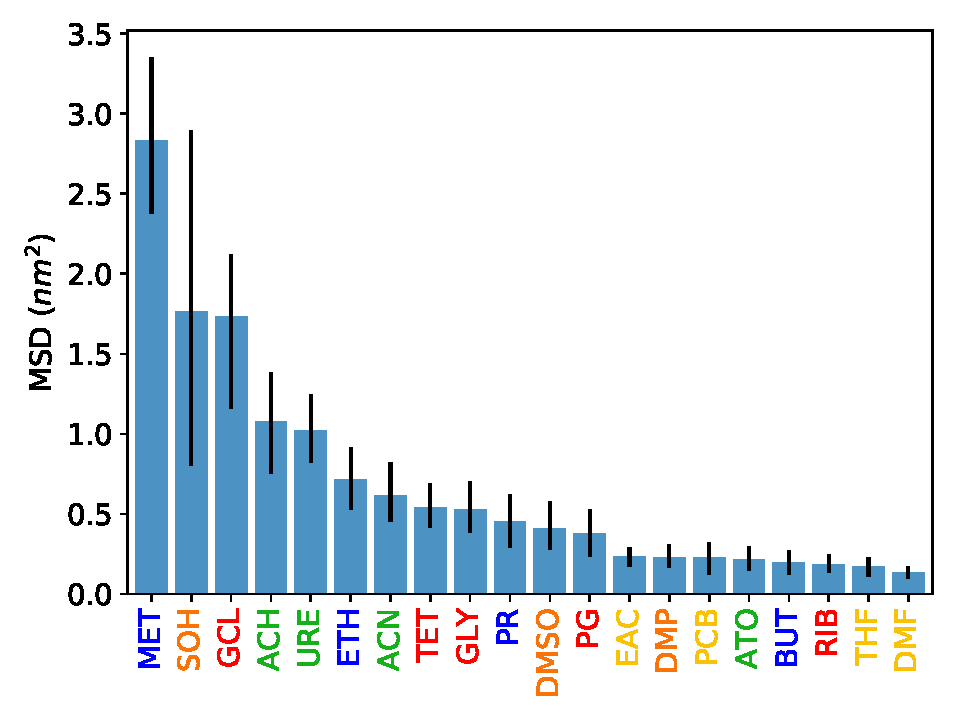
\includegraphics[width=\textwidth]{all_10wt_tamsds.pdf}
  \caption{10 wt \% water}\label{fig:all_msds_10wt}
  \end{subfigure}
  %BJC: missing a few since those simulations just got started
  %BJC1: wondering if I should add some kind of confidence interval to the Stoke-Einstein plots. Based on the errorbars of methanol
  %BJC1: should the points be labeled with residue names?
  \begin{subfigure}{0.45\textwidth}
  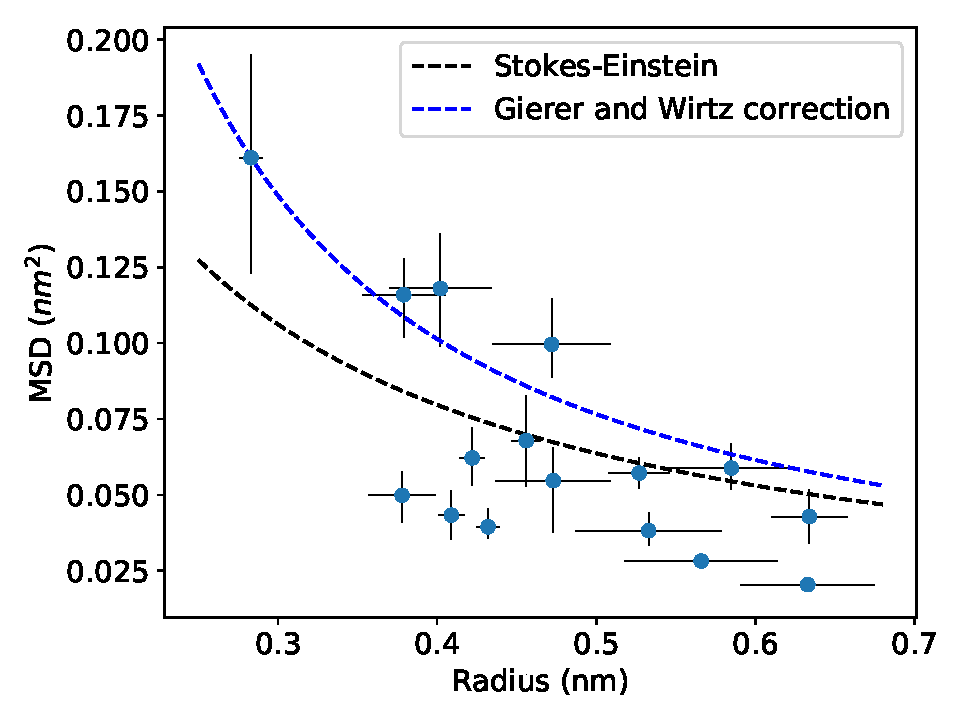
\includegraphics[width=\textwidth]{msd_radius_5wt.pdf} 
  \caption{5 wt \% water}\label{fig:msd_radius_5wt}
  \end{subfigure}
  \begin{subfigure}{0.45\textwidth}
  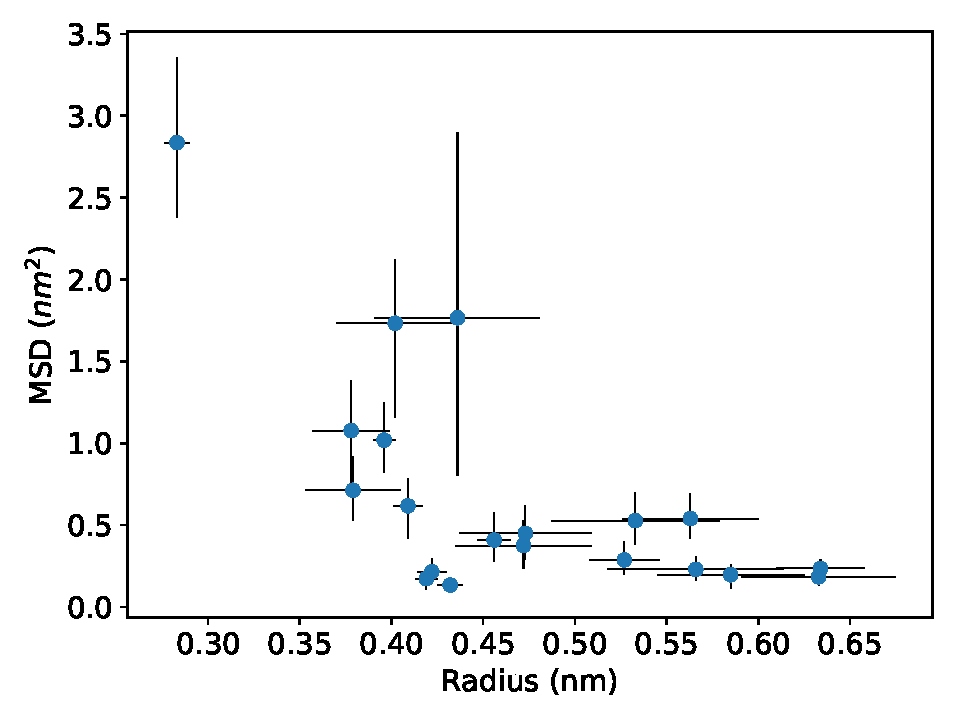
\includegraphics[width=\textwidth]{msd_radius_10wt.pdf} 
  \caption{10 wt \% water}\label{fig:msd_radius_10wt}
  \end{subfigure}
  \caption{The MSDs of solutes in the 5 wt \% water system (a) are significantly
  smaller than those of the solutes in the 10 wt \% water system (b). The
  MSDs are not a monotonic function of molecular size (c and d). A significant
  number of solute MSDs fall below the theoretical lines predicted by the 
  Stokes-Einstein equation and Gierer and Wirtz' corrected Stokes-Einstein equation.}\label{fig:msds}
  \end{figure}  
  %MRS1: Having so much data here grapically is nice. ought to think how else data can be displayed. Perhaps figures with the dwell times as well?  Depends on if those are being shown.  2D scatter plots with average partitioning distance of solute vs. MSD? We should keep brainstorming which will be most relevant. 
  \noindent On the timescales simulated in our study, solutes exhibit subdiffusive behavior.
  %, providing the beginnings of an answer to question~\ref{question:mechanisms}.
  \begin{itemize}  
    \item Figure~\ref{fig:example_ztraces} plots the $z$-coordinate versus time of
  	3 representative ethanol centers of mass in the 10 wt \% water system.
  	\item There are clear periods of entrapment separated by relatively large hops.
	\item The MSD calculated based on all ethanol molecules is plotted in 
	Figure~\ref{fig:example_msd} and is sublinear.
	\item The long periods of entrapment likely lead to this sublinear, and thus
	subdiffusive, behavior.
  \end{itemize}
  
  % Stokes-Einstein underestimates diffusion coefficient for small molecules.
  % r down, f down, D up
  % Stokes-Einstein breaks down for particles less ___ nm in size
  % Fit corrected line through methanol.
  % Make stokes einstein intersect corrected line at breakdown radius
  
  \noindent Solutes partition out of the pore into the head group region and beyond which
  may lead to radially dependent transport mechanisms.
  \begin{itemize}
    \item It is clear from Figure~\ref{fig:example_ztraces} that the longest 
    periods of entrapment usually occur when solutes are far from the pore
    center.
    \item There is a high resistance to movement in the dense head group and
    tail regions.
    \item When hops occur, and where there is the most $z$-positional noise, 
    solutes are generally close to the pore center.
    \item Solutes can move relatively freely when they enter the pore region
    which is primarily composed of water molecules and sodium ions.
  \end{itemize}
  
  \begin{figure}
  \centering
  \begin{subfigure}{0.49\textwidth}
  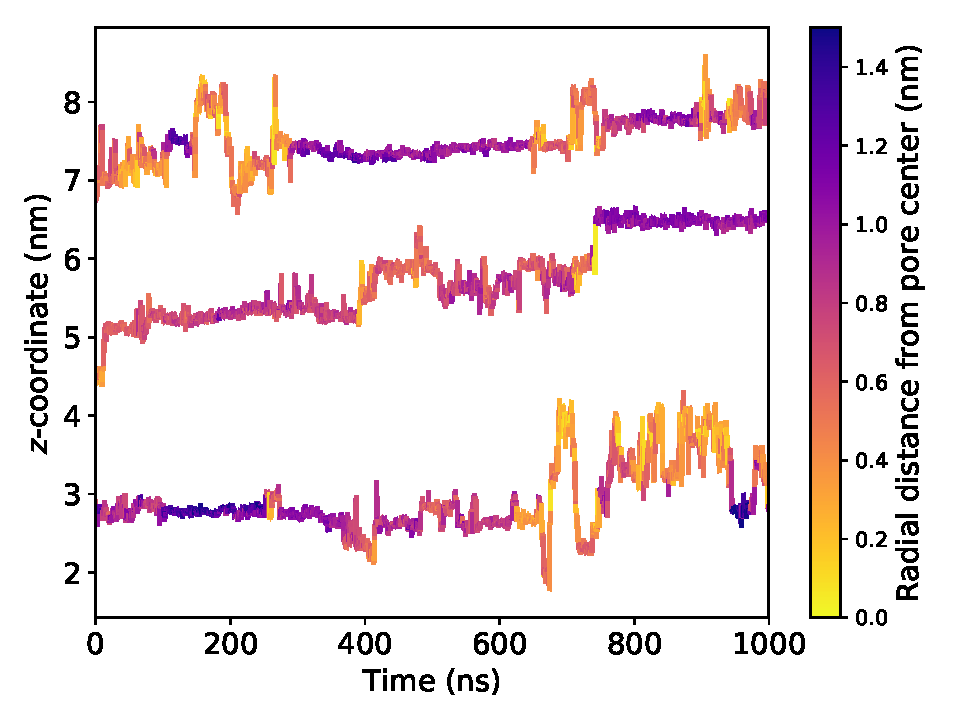
\includegraphics[width=\linewidth]{colorful_example_ztraces.pdf}
  \caption{}\label{fig:example_ztraces}
  \end{subfigure}
  \begin{subfigure}{0.49\textwidth}
  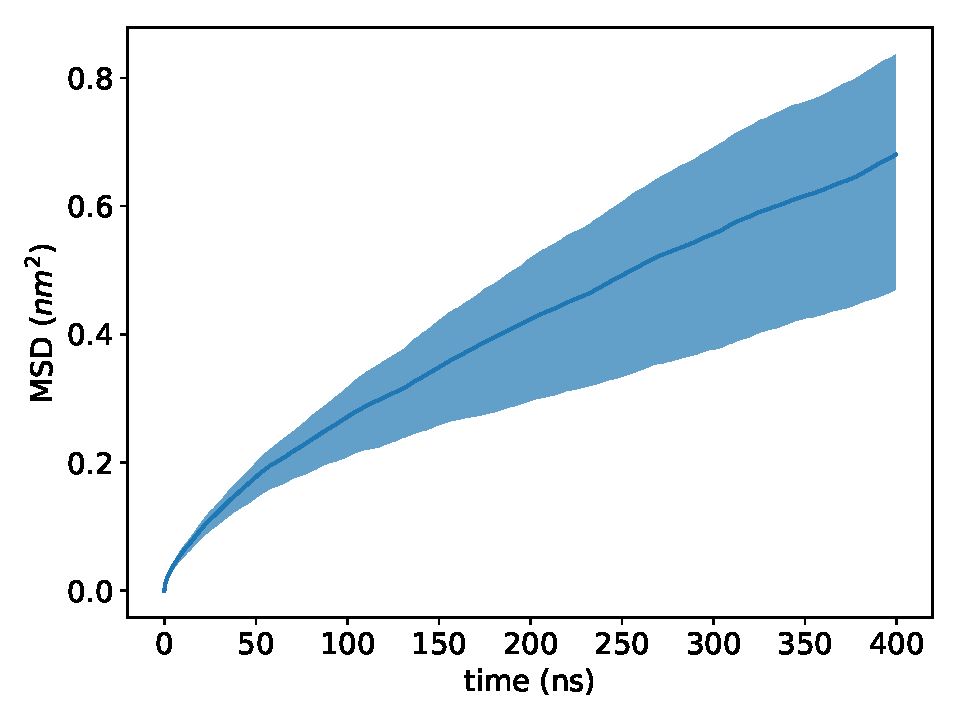
\includegraphics[width=\linewidth]{example_msd.pdf}
  \caption{}\label{fig:example_msd}
  \end{subfigure}
  %MRS1: nice graph!
  \caption{All solutes show subdiffusive transport behavior inside the membrane's
  nanopores, similar to that exhibited by ethanol. (a) The $z$-coordinate trace of
  3 representative ethanol COMs shows clear periods of entrapment separated by hops.
  In general, the longest dwell times occur when solutes are situated far from the
  pore center and the hops occur when solutes are close to the pore center. (b) The
  time-averaged MSD of ethanol is not linear which suggests transport is governed 
  by an anomalous subdiffusion process.}\label{fig:qualitative_mechanisms}
  \end{figure}
  
  In addition to solute trapping in dense monomer regions, we observe a second
  trapping mechanism caused by preferential hydrogen bonding between 
  hydrogen bond donor solutes and monomer head groups. 
  %MRS1: is there a way we can deconvolute these two-three mechanisms?
  \begin{itemize}
    \item To continue with our ethanol example, we observe that the 24 ethanol 
    molecules donate an average of 15.7 hydrogen bonds per frame and accept 
    0.6 hydrogen bonds per frame.
    % BJC1: 6.33 hbonds between EtOH and COOH per frame, 3.84 b/w EtOH and 
    % ether oxygen, 5.56 between EtOH and HOH (where Ethanol donates)
    \item On average, 40 \% of hydrogen bonds donated by ethanol go to 
    carboxylate head groups, 25 \% go to the ether linkages between the tails and
    the head groups and the remaining 35 \% to water.
%    \item This is significant because there are many more water molecules in
%    the pores than there are carboxylate groups.  
%    \item Of the time spent donating hydrogen atom(s), 53 \% of the hydrogen
%    bonds occur between solutes and carboxylate groups as opposed to solutes
%    with water. 
%    \item This shows a high preference for the carboxylate anions since there
%    are 5 times more water molecules in the system.  % BJC1: more like 3 times more water molecules because many are in the tails.
    %MRS1: carboxylate also has net negative charge - not just higher negative partial charge,
    %also no extra neutralizing positive partial charge nearby.
    \item There are less carboxylate oxygen atoms in the pore than there are water
    molecules yet more hydrogen bonds are donated to them.
    \item The stability of hydrogen bonds with carboxylate oxygen atoms is likely
    high since the oxygen atoms have a negative charge with no neutralizing positive
    charges nearby.
    \item Additionally, on average, each sodium ion is coordinated to 1.7 water
    molecules meaning an appreciable fraction of the water molecules occupying 
    the pore region are usually coordinated to a sodium ion which decreases 
    their availability to accept hydrogen bonds from solutes.
    % MRS1: this should lead to reduced ability to solvate positive things, but 
    % shouldn't reduce H-bonding that much?
    % BJC1: I think that it takes away acceptor oxygen atoms since they are occupied
    % by sodium. The hydrogen atoms of water could still hbond but I'm just talking
    % about ethanol donating to water, for which opportunities should be suppressed.
  \end{itemize}
  
  Finally, we see instances of solutes that become immobilized or slowed by 
  association with sodium counterions. 
  \begin{itemize}
    \item Much like water, the polarity of the solutes creates regions of high
    electron density, modeled using partial negative charges, which are stabilized
    through electrostatic interactions with sodium ions.
    \item There are many cases in which polar groups bind to sodium ions for at
    least a short period of time. 
    \item There are some cases where solutes become immobilized for long periods
    of time while in close proximity to a sodium ion.
    \item In Figure~\ref{fig:na_met_trace}, the oxygen atom of methanol stays
    within 2.5 \AA~of a sodium ion for the entire length of a trapping occurence.
  \end{itemize}
  
  \begin{figure}[!htb]
  \centering
  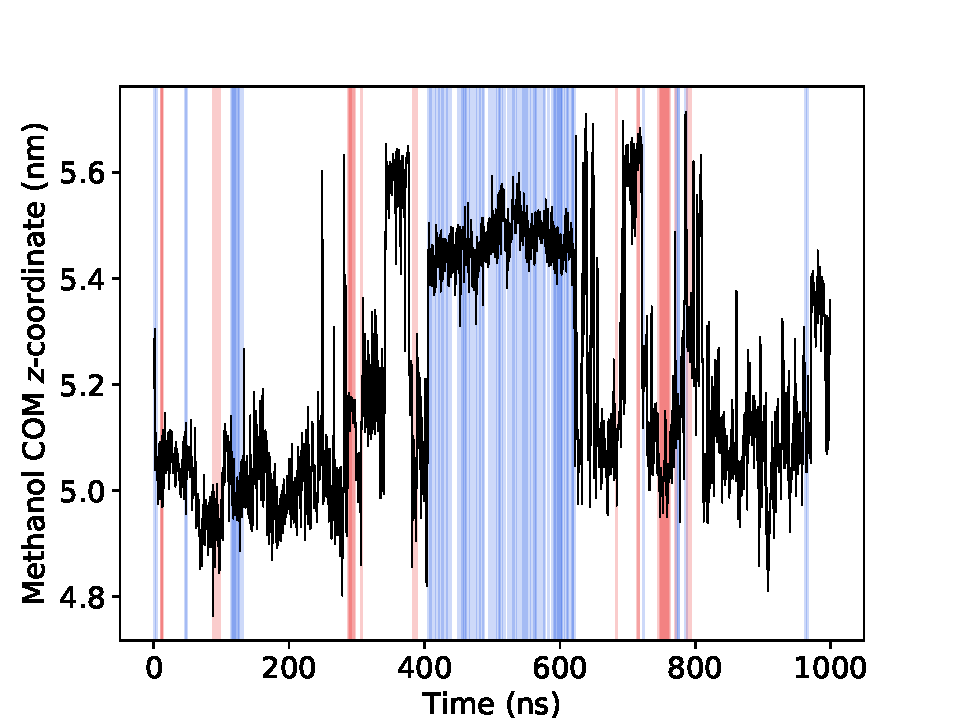
\includegraphics[width=0.45\textwidth]{na_met_trace.pdf}  % create with nn.py located in MET/10wt
  \caption{The oxygen atom of methanol stays within 2.5 \AA~of the same sodium ion for
  the majority of the trapping occurence between 400 and 600 ns. Regions
  highlighted red or blue indicate times when methanol's oxygen atom is within 
  2.5 \AA~of a sodium ion. The color of the shaded regions are switched every time
  the oxygen atom becomes associated to a different sodium ion.}\label{fig:na_met_trace}
  \end{figure}

  %MRS1: I think maybe we want to keep this minimal. 
  %BJC1: Leaving out for now
%  \noindent The hopping and trapping mechanism exhibited by all solutes is characteristic of
%  a continuous time random walk (CTRW) model.	
%  \begin{itemize}
%  	\item The length of entrapment follows a power law distribution 
%  	(Figure~\ref{fig:example_powerlaw}) and the distribution of hop lengths can be 
%  	described with a Gaussian distribution (Figure~\ref{fig:example_hop_dist}).
%  	\item Power law distributed dwell times are responsible for the ageing phenomenon
%  	which causes the slope of the MSD curve to decrease with increasing measurement
%  	time because longer dwell times are sampled.  %BJC: might need to reword this a bit 
% 	\item Although these observed distributions strongly support a CTRW model, the time-averaged
% 	MSD of a pure CTRW should be linear which is not the case.~\cite{neusius_subdiffusion_2008,meroz_subdiffusion_2010}
%  \end{itemize}
%  
%%  \noindent The direction of each hop is anti-correlated to the direction of the previous hop.
%  \noindent Transport may be better described by a subordinated fractional brownian motion 
%  (sFBM) model.
%  \begin{itemize}
%  	\item Figure~\ref{fig:example_autocovariance} shows the autocovariance function of 
%  	ethanol step vectors. % BJC: vectors because includes magnitude + direction. Is there a better word?
%  	\item The negative autocovariance at low values of k indicates anti-correlation
%  	between hops. 
%  	\item If solutes followed a pure CTRW mechanism, the autocovariance function would
%  	decay to zero immediately.
%  	\item Although the autocovariance function is relatively noise, due to the somewhat small
%  	number of hops observed over the course of each solute trajectory, there is the least 
%  	uncertainty at k=1, the most insightful data point. This behavior is consistent across
%  	all solutes molecules. % Can put error bars on points
%  	\item Therefore, we believe transport can be described as subordinated fractional Brownian
%  	motion where the leading process is a CTRW with hops whose direction is dictated by the parent
%  	process, FBM.
%  	\item Future publications will focus on modeling the solute's transport characteristics
%  	with an sFBM model
%  	\item We will draw on these observations only in a qualitative sense for the remainder of this work.
%  \end{itemize}
%  
%  %BJC: seems like the MSD becomes linear at long times. Perhaps due to loss of memory with time.
%
%  \begin{figure}
%  \centering
%  \begin{subfigure}{0.325\textwidth}
%  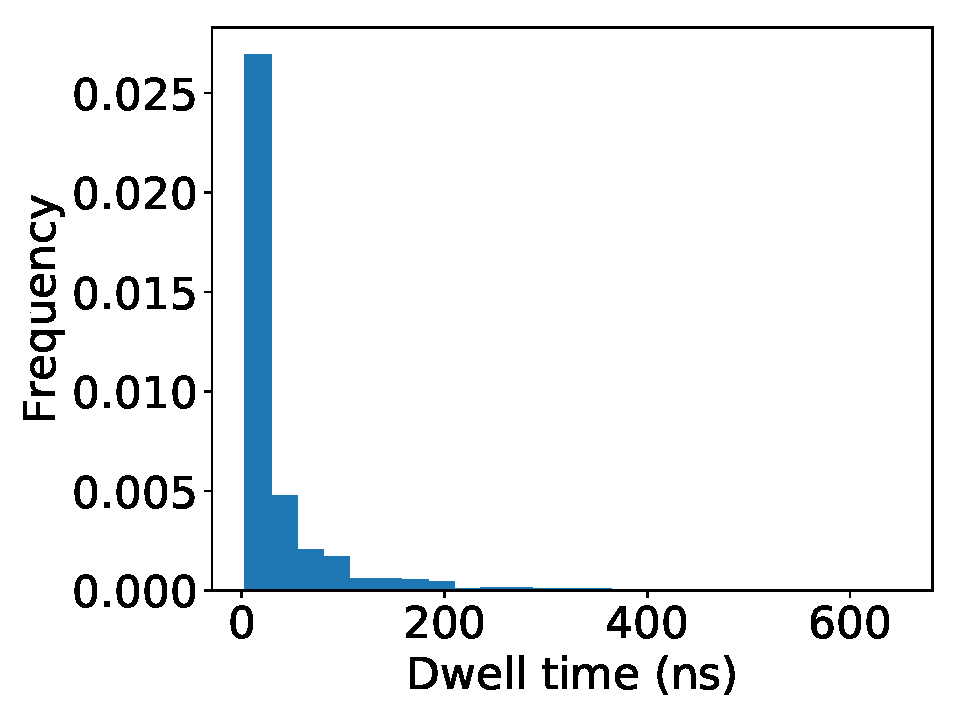
\includegraphics[width=\linewidth]{example_powerlaw.pdf}
%  \caption{}\label{fig:example_powerlaw}
%  \end{subfigure}
%  \begin{subfigure}{0.325\textwidth}
%  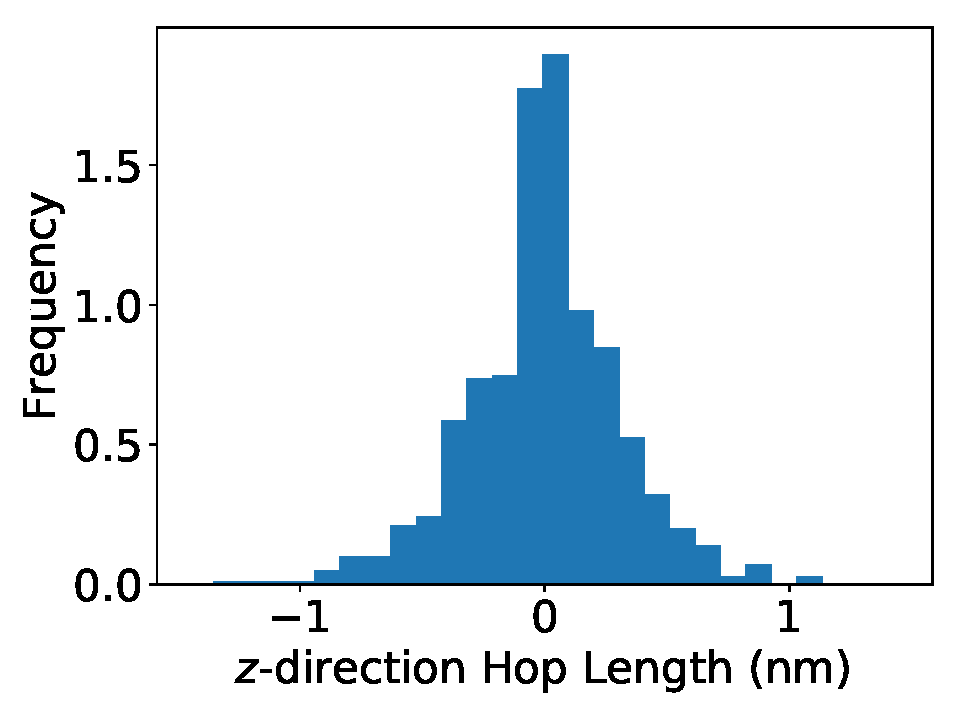
\includegraphics[width=\linewidth]{example_hop_dist.pdf}
%  \caption{}\label{fig:example_hop_dist}
%  \end{subfigure}
%  \begin{subfigure}{0.325\textwidth}
%  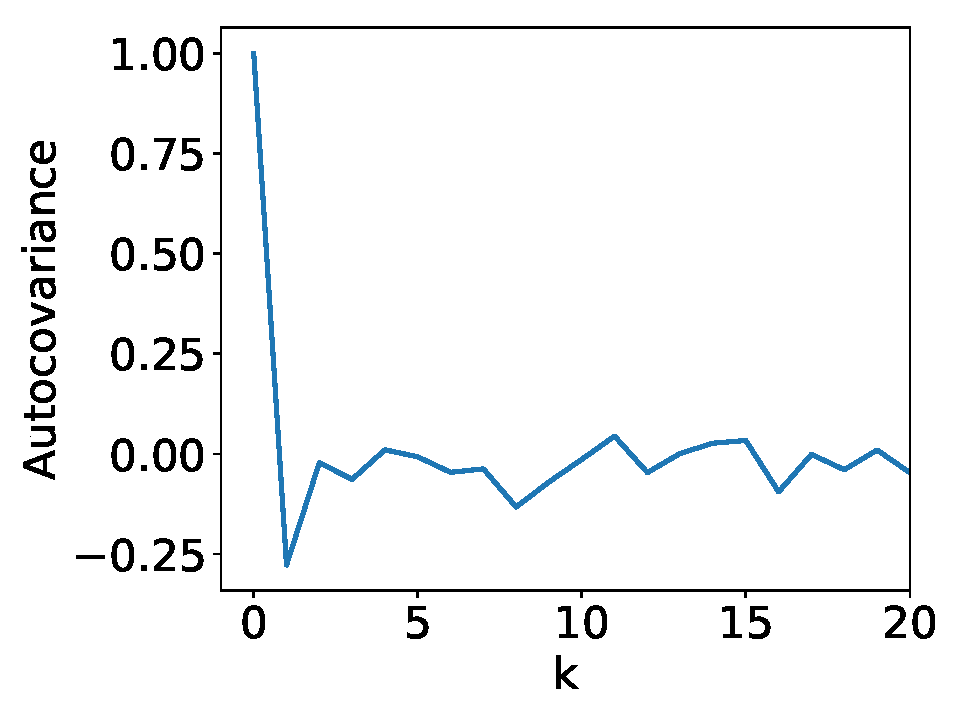
\includegraphics[width=\linewidth]{example_autocovariance.pdf}
%  \caption{}\label{fig:example_autocovariance}
%  \end{subfigure}
%  \caption{(a) The distribution of dwell times resembles a power law distribution. 
%  (b) The distribution of hop lengths appears Gaussian. (c) Hops are anti-correlated
%  to their previous hop as indicated by the negative value of the autocovariance 
%  function at $k$ = 1.}\label{fig:examples}
%  \end{figure}
  
  \noindent The transport behavior exhibited by solutes in the 5 wt \% water systems
  is similar to that shown by those in the 10 wt \% system however the timescales are
  much longer.
  \begin{itemize}
    %BJC: will put supporting data in supporting information
    \item We observe subdiffusive behavior with intermittent hopping between
    periods of entrapment.
    \item The frequency and length of hops are both diminished in the 5 wt \% system.
    \item Since there are only 24 solute molecules in each system, in order to obtain
    better time-averaged descriptions of solute transport mechanisms, we will focus
    the rest of our analysis on transport in the 10 wt \% water systems.
  \end{itemize}
  
%  We will revisit our observations in the the context of specific groups of 
%  molecules in the discussion that follows.
  
%  \noindent The MSDs in Figure~\ref{fig:all_msds} are a strong function of two solute 
%  trapping mechanisms.
%  \begin{itemize}
%  	\item Solutes that are hydrogen bond donors can be stabilized through hydrogen bonds
%  	with one of the five oxygen atoms attached to each monomer head group. 
%  	\item In a separate interaction, solutes can become kinetically trapped between or behind
%  	monomer head groups. These interactions likely lead to the observed anti-correlated
%  	hopping	behavior.
%  	\item Generally, both mechanisms affect each solute to varying degrees.
%  \end{itemize}
  
  %BJC: This will need updating once all the rest of outline is written.
%  \noindent The degree to which solutes are influenced by each entrapment mechanism
%  is a complex function of a solute's size, shape, and polarity.
%  \begin{itemize}
%    \item In general, solutes can move fastest in the pore center, where
%    there is comparatively little resistance to diffusion.
%	\item The 5 fastest solutes in our study have a low molecular weight and
%	spend a significant amount of time in the pore center. They are only slowed
%	by hydrogen bonds with monomer carboxylate groups.
%	\item Bulky solutes with many hydrogen bond donating groups, like glycerol,
%	spend most of their time in the pore center, but their large size combined
%	with a higher solute-head group hydrogen bond frequency, makes their dynamics slow. 
%    \item Solutes with high hydrophobic character tend to partition into the 
%    head group region where entrapment occurs.
%    \item We observe low MW solutes with lower-than-expected MSDs because they
%    spend more time trapped between monomer head groups due to low water
%    solubility.
%    \item Small, planar molecules, without the ability to donate hydrogen bonds, like acetone,
%    exhibit some of the slowest MSDs. Their flat geometry and small size makes it easy for 
%    them to get lodged deep between head groups.
%  	\item Overall solutes exhibit some degree of trapping, by one or a combination of the above
%  	mechanisms, with anticorrelated hops between each period of immobility due to 
%  	obstructions.
%  \end{itemize}
  
  %BJC: potential figure to go with above paragraph
  % (a) Plot showing how biggest jumps are at pore center
  % (b) Illustrate preference for hbonds carboxylate head groups

%  We will explore these factors in greater detail in the context of 
%  specific groups of molecules in the discussion that follows.

% BJC: Move to supporting
%  \subsection*{Transport of Water}
%
%  The MSD of water is a weak function of the solute residue disolved in
%  the pores.
%  \begin{itemize}
%  	\item Large molecules like glycerol and ribose obstruct the movement
%  	of water molecules forcing them to have lower MSDs
%  	\item I don't know why the MSD is fast in the fastest systems or why DMSO is slow.
%  	\item Sulfur containing compounds have slowest water transport
%  	\item How do 24 solute molecules have such a drastic effect on water motion
%  \end{itemize}
%
%  % BJC: MSDs only calculated for water molecules that spend > 95 % of their
%  % time in the pore. Pore region / tail region cutoff is at 1.5 nm (approximate location of lowest radial water density) 
%  \begin{figure}
%  \centering
%  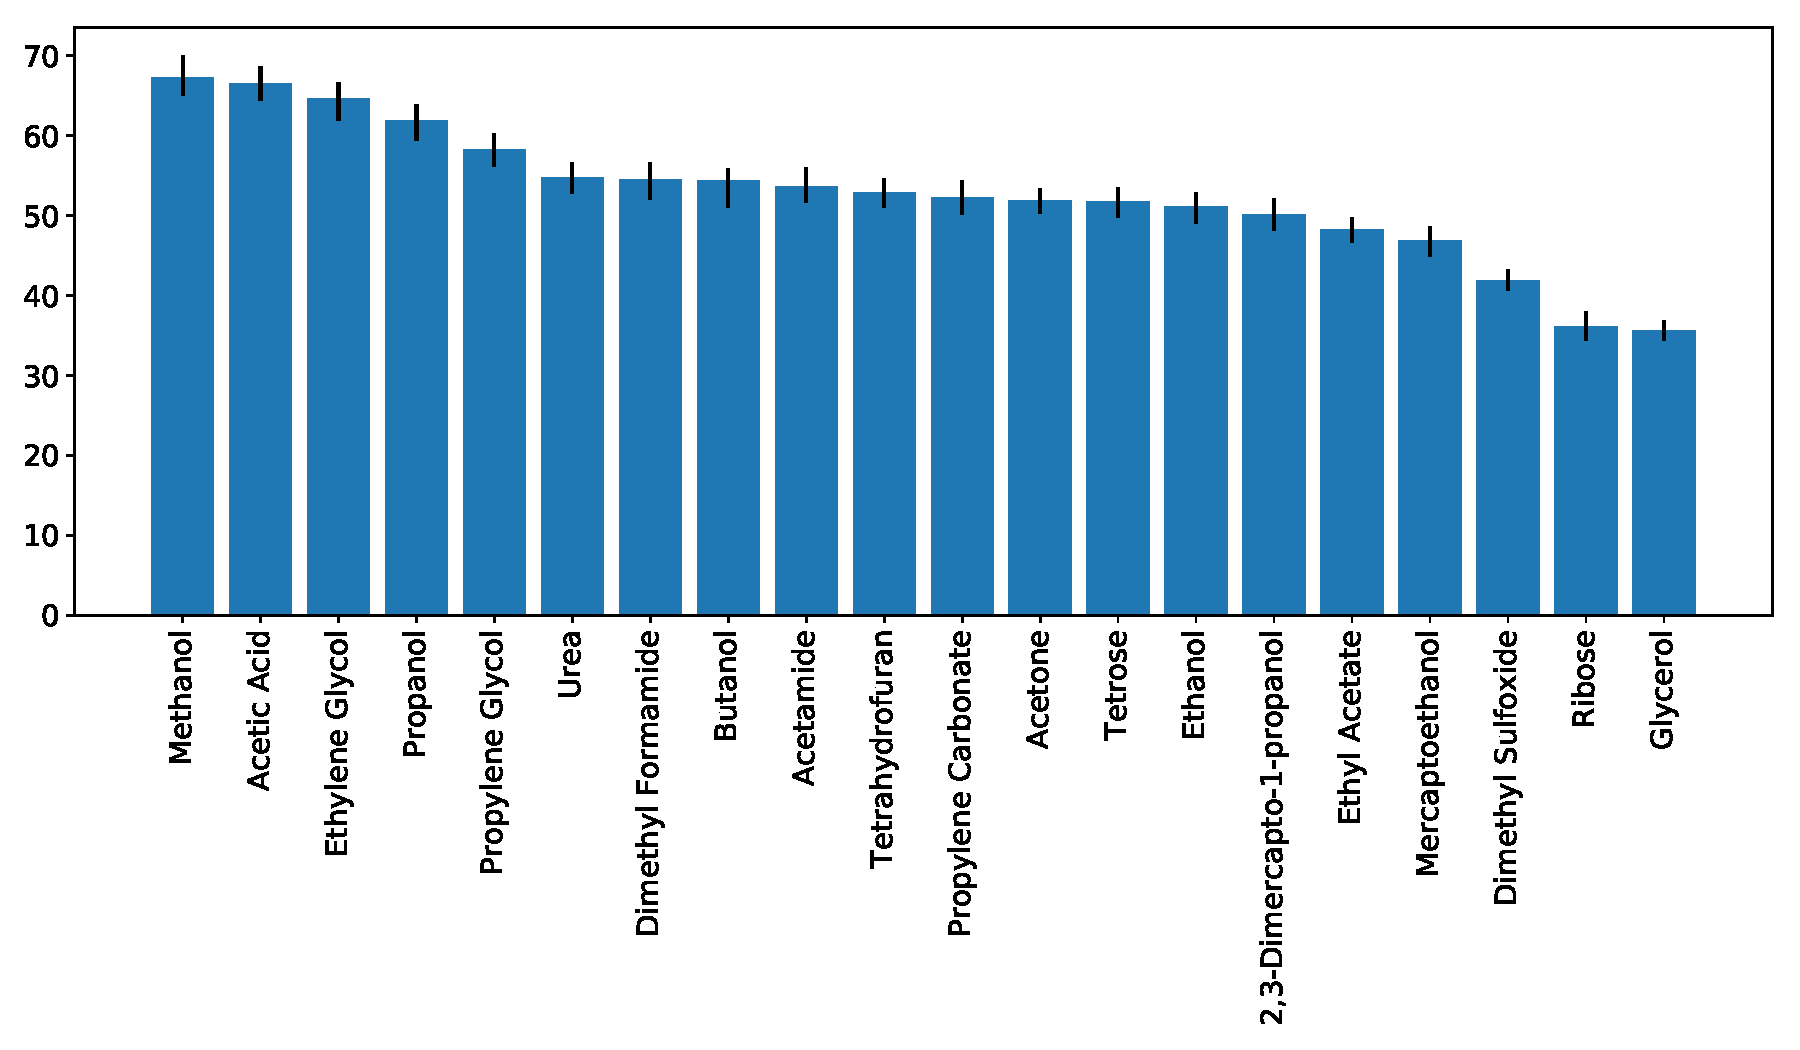
\includegraphics[width=\textwidth]{water_msd.pdf}
%  \caption{}\label{fig:water_msd}
%  \end{figure}
  
  % BJC. Other Notes:
  % There is no discernable trend in flux of water to/from pores. Most levels stay 
  % comparable to their initial values while a handful have ~50 water molecules that
  % enter the pore during the simulation.
  % Water molecules that spend > 95 % of their time within 1 nm of the pore center 
  % have lower MSDs -- although there aren't a lot of them to average over. They are
  % probably lower because they can't be moving much to stay so confined
  
  % General framework for following sections
  % The MSDs are in this order. This is counterintuitive / makes sense for some reason
  % Here are the RDFs
  % Here is some other feature that helps explain things.
  
  \subsection*{Transport of Simple Alcohols}

%  The MSD of methanol, ethanol, propanol and butanol descends in order of 
%  their size, however, the.
%  \begin{itemize}
%    \item The MSD of ethanol, propanol and butanol descend approximately
%    linearly as expected from the Stokes-Einstein relationship  % BJC: maybe better to use wilke-chang version with correction factor
%    \item However, methanol travels considerably faster than suggested by the
%    relationship. (See Figure~\ref{fig:msd_radius_simple_alcohol_rdf}
%  \end{itemize}    

  The MSDs of methanol, ethanol, propanol and butanol descend in order of 
  their size.
  \begin{itemize}
    \item Using methanol as a reference, the other alcohols move slower than
    expected according to both the pure Stokes-Einstein relationship and the
    corrected relationship (See Figure~\ref{fig:msd_radius_simple_alcohol_rdf}).
  \end{itemize}   
  
  Methanol moves fast, not only because it is the smallest solute studied in this work, but
  because it has the highest radial density near the pore center where the largest hops occur.
  \begin{itemize}
    \item The radial density as a function of distance from the pore center
    for each alcohol is plotted in Figure~\ref{fig:simple_alcohol_rdf}.
    \item On average, the density of methanol in the pore center is only slightly
    less than the density near the head groups.
    \item All other alcohol molecules are most concentrated in the head group region.
  \end{itemize}
  
  All simple alcohols participate in a similar number of hydrogen bonding interactions
  with the monomer head groups, but with varying preference towards hydrogen bonds with
  the monomer carboxylate oxygen atoms over the ether oxygen atoms (See Figure~\ref{fig:simple_alcohol_hbonds})
  % caused by increasing hydrophobic character.
  \begin{itemize}
  	\item If all 5 hydrogen bonding acceptor sites on the monomer head groups were equal,
  	we would expect the ratio of the number of hydrogen bonds between solutes and the two 
  	carboxylate oxygen atoms to the number of hydrogen bonds between solutes and the three
  	ether groups to be 2/3. 
  	\item There is a clear preference towards hydrogen bonding with the carboxylate 
  	oxygen atoms for all simple alcohols.
  	\item This is largely due to the large net charge of the carboxylate groups as well
  	as the more highly crowded environment surrounding the ether oxygen atoms. % combined with their lower electron density. % partial charges.
  	\item Butanol shows the largest preference towards hydrogen bonds with carboxylate 
  	head groups.
  	\item The radial distribution function of atoms located at opposite ends of butanol
  	shows that, on average, oxygen atoms are situated 0.25 nm closer to the pore centers
  	than the distal carbon atoms.
  	\item This suggests that alcohols tend to orient themselves like the liquid crystal 
  	monomers, with hydrophilic components point towards the pore centers.
  	%\item When solutes are buried in the pore walls, their MSDs are shorter.
  \end{itemize}
  
  \begin{figure}
  \centering
  %BJC1: I'm not sure of figure (a) is necessary
  \begin{subfigure}{0.45\textwidth}
  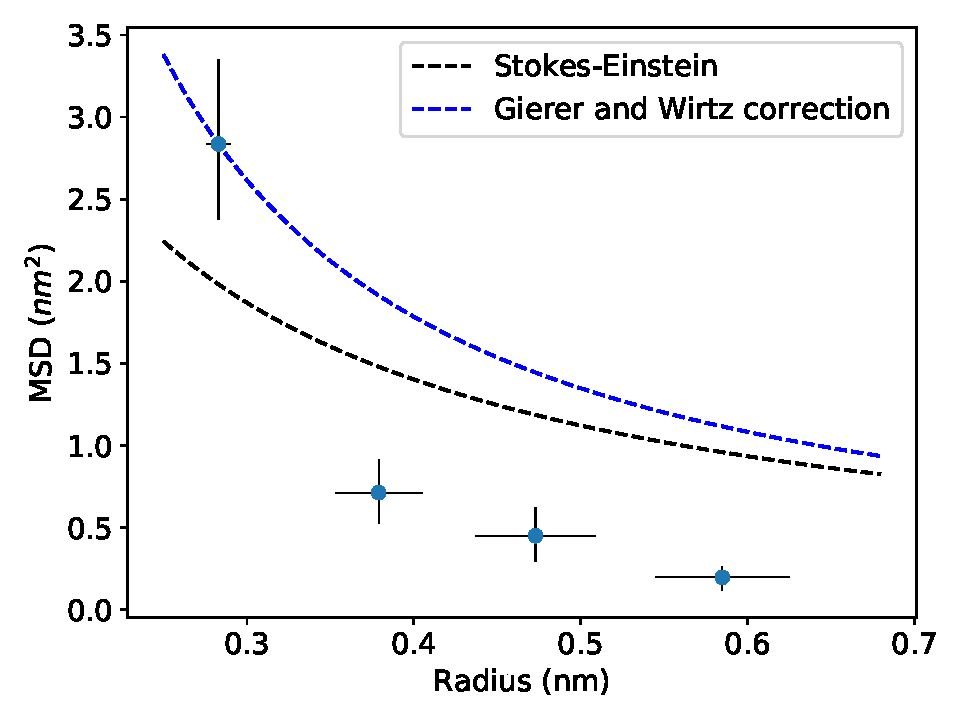
\includegraphics[width=\linewidth]{msd_radius_simple_alcohols_10wt.pdf}
  \caption{}\label{fig:msd_radius_simple_alcohol_rdf}
  \end{subfigure}
  \begin{subfigure}{0.45\textwidth}
  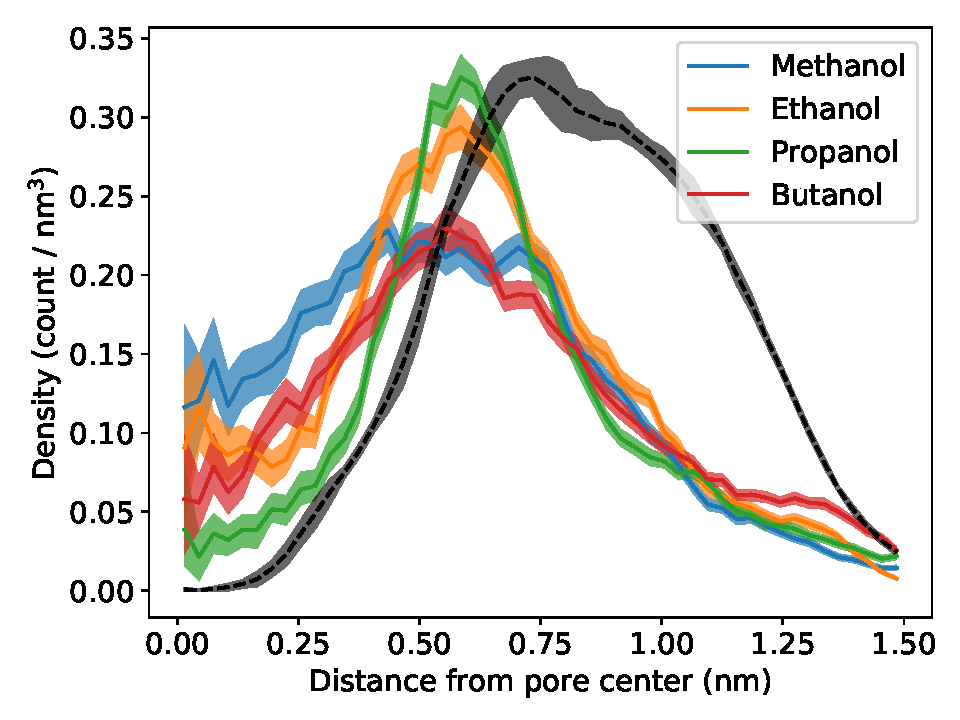
\includegraphics[width=\linewidth]{simple_alcohol_rdf.pdf}
  \caption{}\label{fig:simple_alcohol_rdf}
  \end{subfigure}
  \begin{subfigure}{0.45\textwidth}
  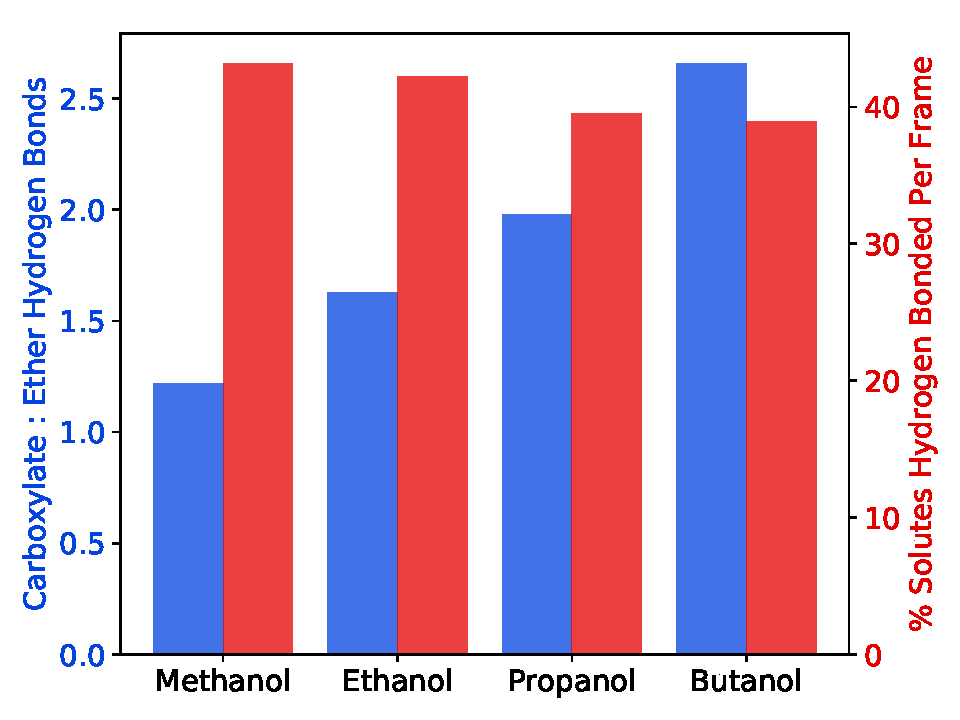
\includegraphics[width=\linewidth]{simple_alcohol_hbonds.pdf}
  \caption{}\label{fig:simple_alcohol_hbonds}
  \end{subfigure}
  \begin{subfigure}{0.45\textwidth}
  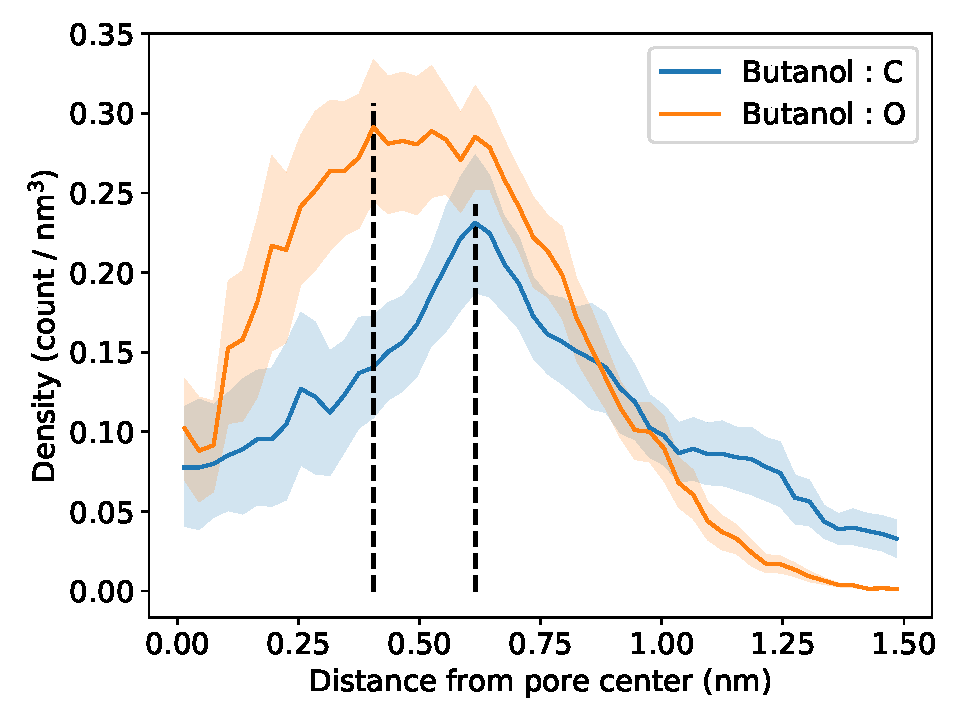
\includegraphics[width=\linewidth]{butanol_CO.pdf}\lapbox[\width]{-2.85cm}{\raisebox{3cm}{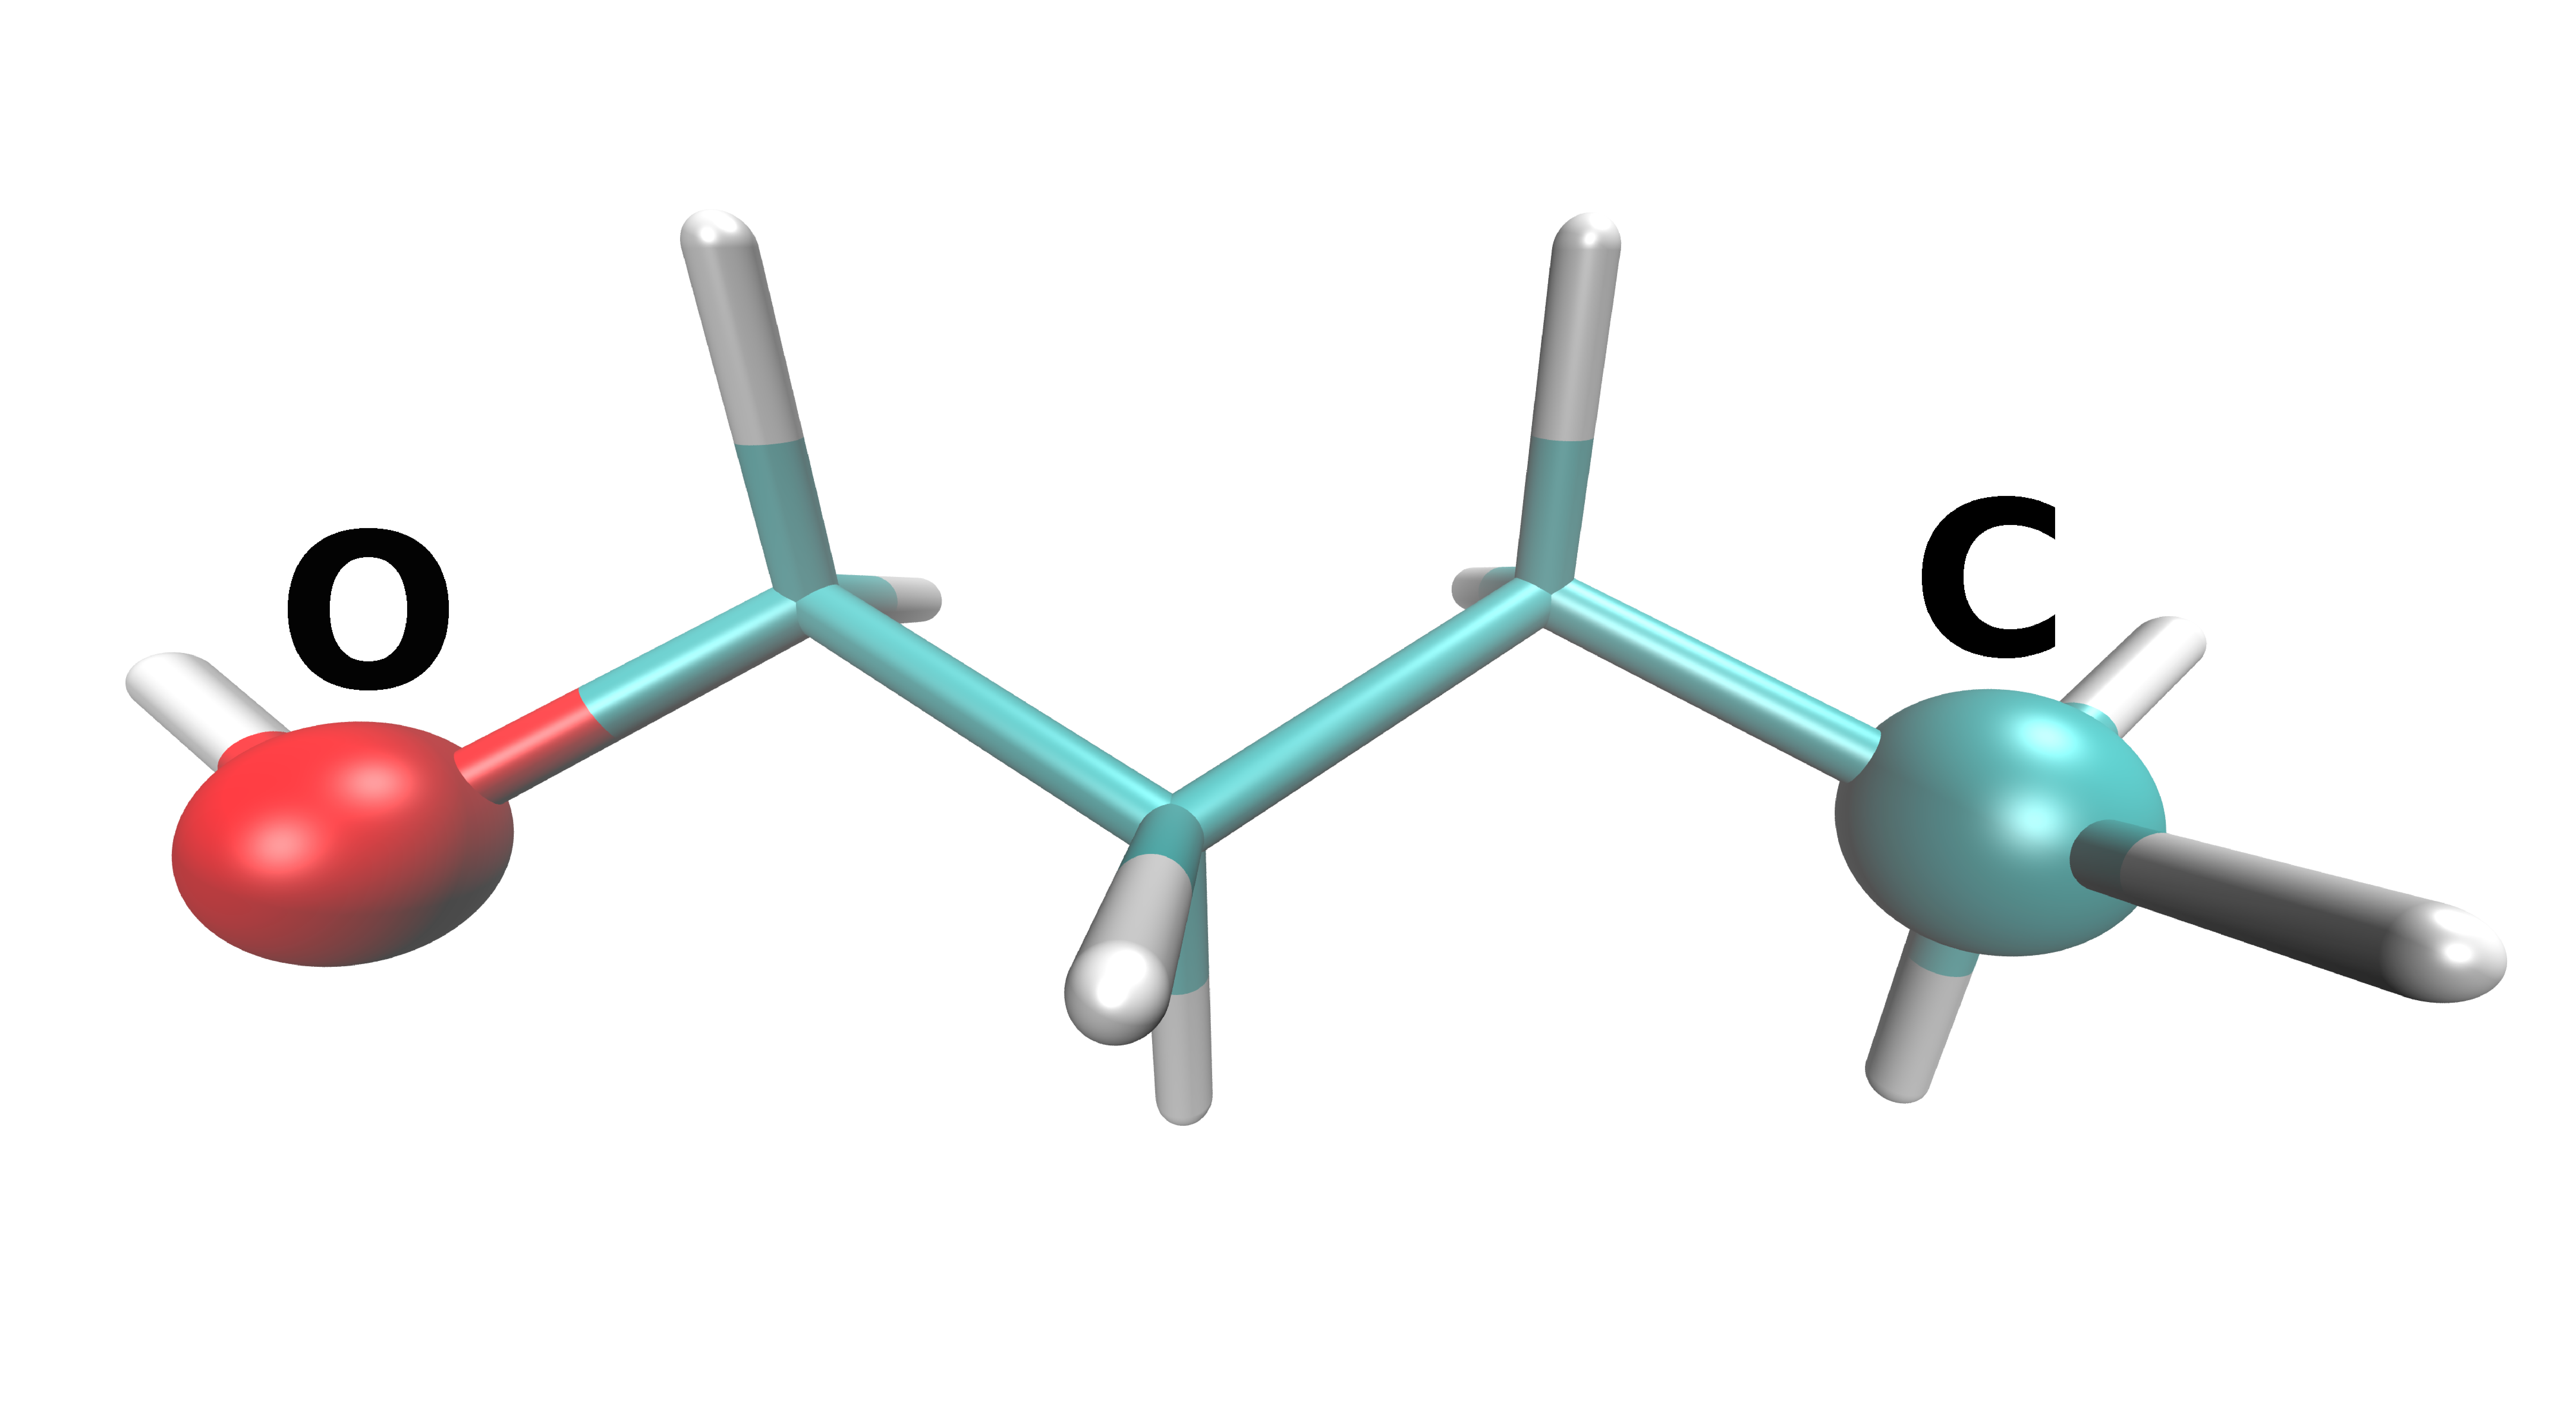
\includegraphics[height=1.4cm]{butanol_labeled.pdf}}}
  \caption{}\label{fig:butanol_CO}
  \end{subfigure}
  %MRS: label the black line (tails? heads?)
  \caption{(a) The MSD of the simple alcohols decrease as a function of the solute size, however
  methanol's MSD is considerably higher than expected based on the Stokes-Einstein equation. 
  (b) The radial distribution functions of each simple alcohol shows a maximum close
  to the highest density of monomer head groups (dashed line, normalized for easier visual
  comparison). Methanol spends the largest proportion of time, relative to the other alcohols,
  near the pore center, which may help explain its fast dynamics. (c) Despite relatively little
  difference in the total number of active hydrogen bonds per frame, a given alcohol's preference
  towards hydrogen bonds with the carboxylate groups increases with molecule size. (d) The average
  location of butanol's oxygen atom is significantly closer to the pore center than its most distal
  carbon atom, suggesting that the molecule is oriented with hydrophobic tails pointing away from
  the pore center.}\label{fig:simple_alcohols}
  \end{figure}

  \subsection*{Transport of Diols, Triols and Sugars}  % polyols instead of sugars?
  
  The order of the MSDs of solutes in this grouping are roughly consistent with 
  their size, however propylene glycol moves exceptionally slow.  %BJC: or tetrose and glucose are exceptionally fast
  \begin{itemize}
  	\item Ethylene glycol has the highest MSD followed by tetrose
  	and glycerol, whose MSDs are similar, propylene glycol, the second smallest
  	solute of this set, and finally ribose.
  \end{itemize}
  
  Transport is both facilitated and hindered by additional solute hydroxyl groups
  due to their influence on radial density and hydrogen bond frequency.  	
  \begin{itemize} 
    \item Extra hydroxyl groups cause solutes to favor the water-rich pore region.
    where there is the least hindrance to movement (See Figure~\ref{fig:polyols_rdf}).
    \item Tetrose, ribose and glycerol are densest close to the pore center. This is 
    likely a result of their hydrophilicity and large size which prevents them from
    partitioning into the head group region.
    \item However, these extra hydroxyl groups facilitate a larger number of 
    hydrogen bond interactions that work to hold solutes in place (See Figure~\ref{fig:multi_hbonds}).
    \item It has been observed that hydrogen bonding in a system will generally
    reduce diffusivity~\cite{srinivas_computer_1999}
%    \item Ethylene glycol, the fastest solute in this grouping (and second fastest
%    overall), obtains the best balance of both effects.
  \end{itemize}
  
  The number of hydrogen bonding interactions between solutes and head groups
  increases with the number of solute hydroxyl groups.
  \begin{itemize}
    \item These solutes frequently undergo simultaneous hydrogen bond interactions as
    shown in Figure~\ref{fig:multi_hbonds}. 
    \item For example, both hydroxyl groups of ethylene glycol can undergo hydrogen
    bonds with different hydrogen bond acceptors at the same time.
    \item In some cases, all 4 hydroxyl groups of ribose are hydrogen bonded to monomer
    head groups simultaneously.
    \item Hydrogen bonds act as a kind of molecular glue which holds solutes in place, 
    especially when there are many, however proximity to the pore center partially 
    compensates for this effect in the cases of glycerol and tetrose.
  \end{itemize}
  
  \begin{figure}[!htb]
  \centering
  \begin{subfigure}{0.45\textwidth}
  % BJC: This might be better cut off at y ~ 0.6 and then provide an inset with full RDFs
  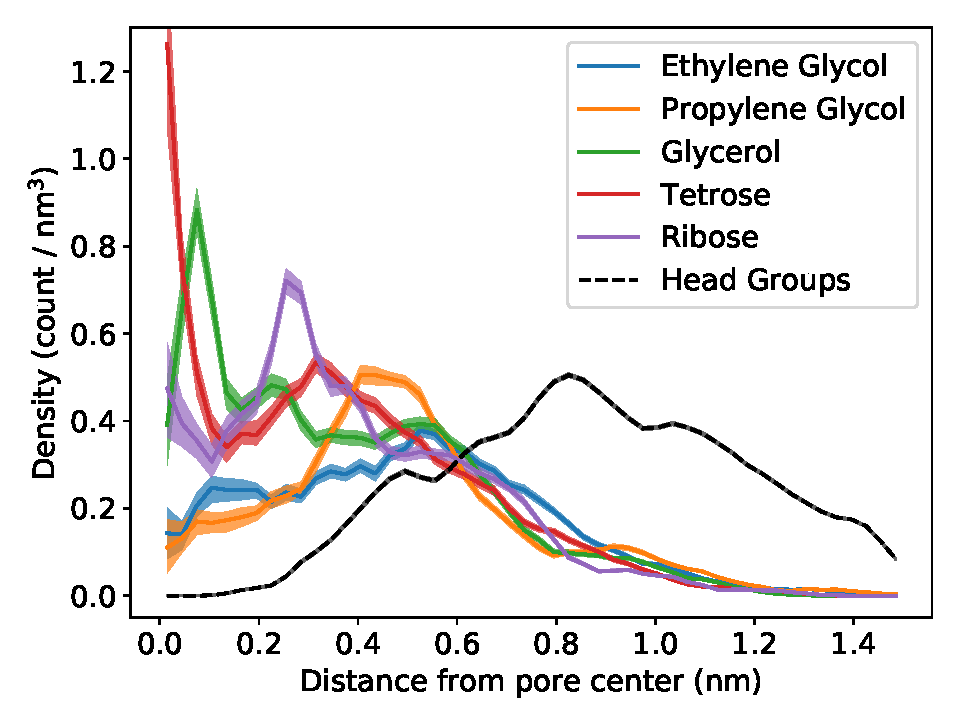
\includegraphics[width=\linewidth]{polyols_rdf.pdf}
  \caption{}\label{fig:polyols_rdf}
  \end{subfigure}
  \begin{subfigure}{0.45\textwidth}
  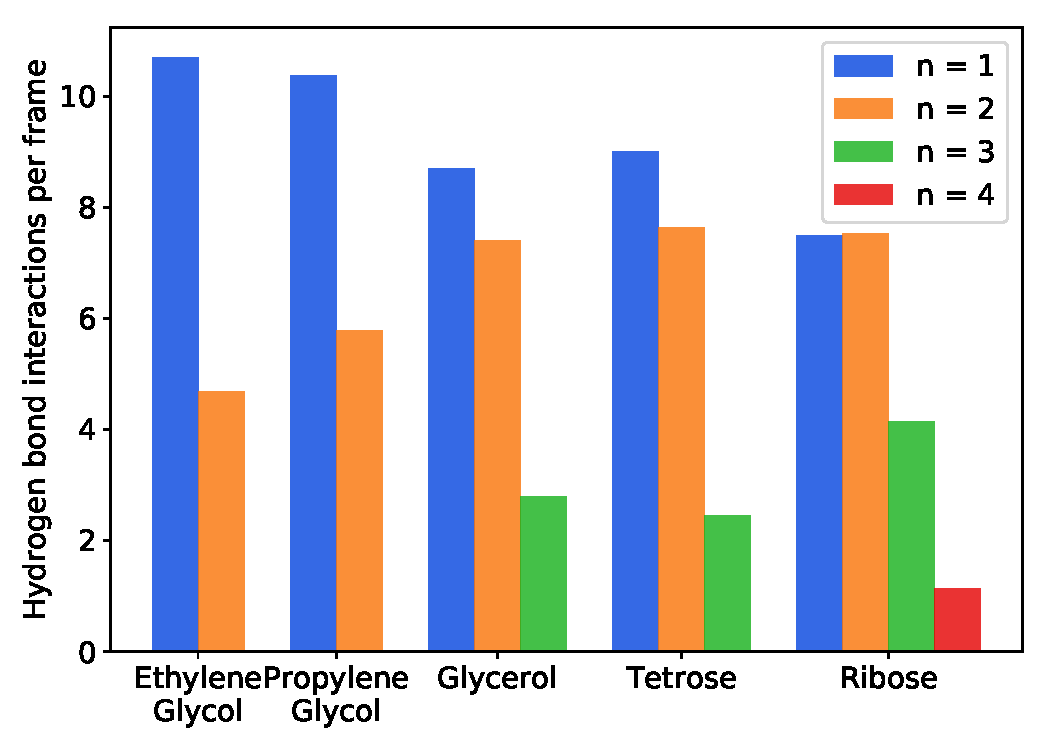
\includegraphics[width=\linewidth]{multi_hbonds.pdf}
  \caption{}\label{fig:multi_hbonds}
  \end{subfigure}
  % BJC: this subfigure is probably best suited for the supporting information.
%  \begin{subfigure}{\textwidth}
%  \centering
%  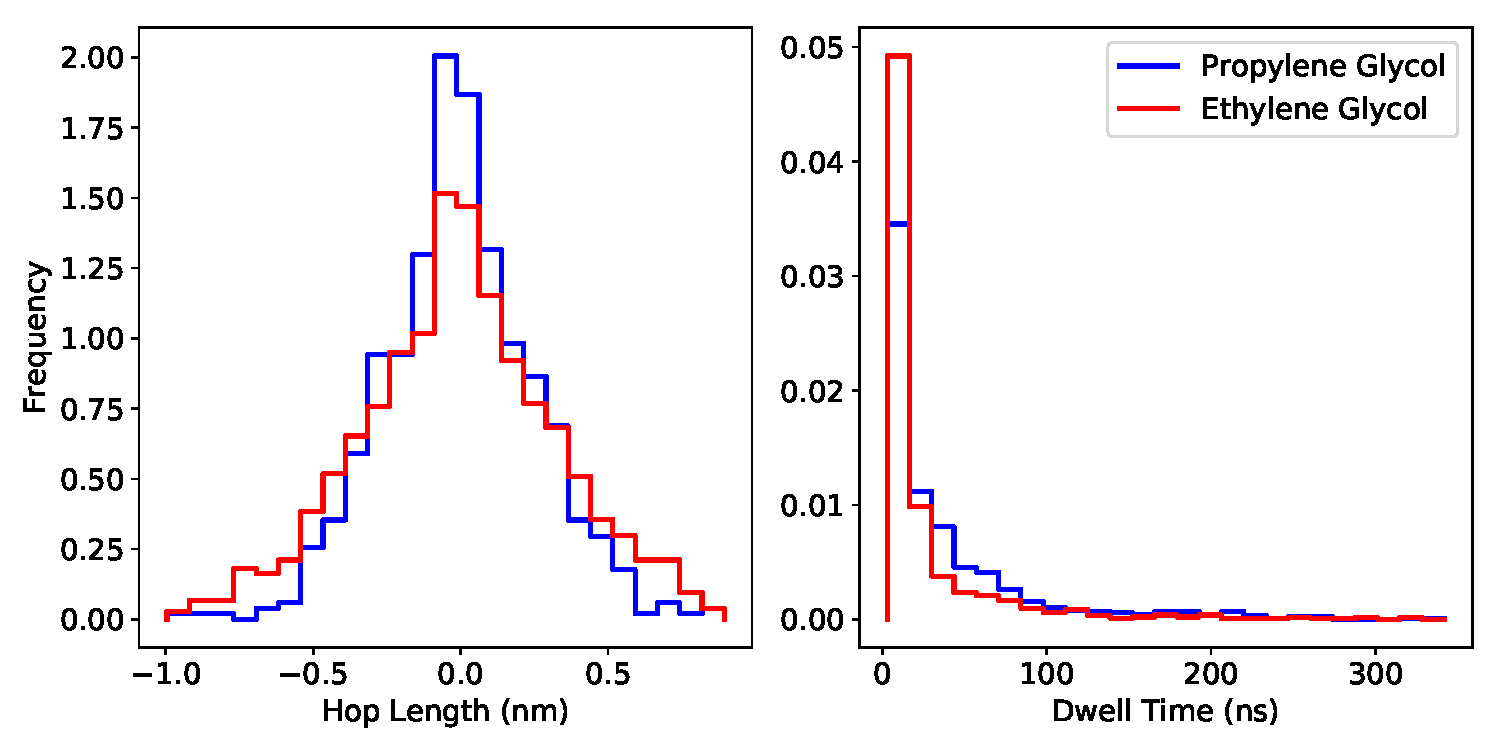
\includegraphics[width=0.9\linewidth]{dwell_hop_PG_GCL.pdf}
%  \caption{}\label{fig:dwell_hop_PG_GCL}
%  \end{subfigure}
  \caption{(a) Glycerol, tetrose and ribose are densest close to the pore center because
  they have a high number of hydrophilic groups and are relatively large. Ethylene glycol
  and propylene glycol are densest close to the head group region. (b)The number of 
  hydrogen bond interactions between solutes and monomers increases as solutes gain additional
  hydroxyl groups. Often, multiple hydroxyl groups within a solute often hydrogen bond in
  different locations simultaneously. Occasionally, all four hydroxyl groups
  of Ribose (n = 4) are involved in a hydrogen bond interaction at the same time.}\label{fig:multi_hbonds}
  \end{figure}
  
  Of the two diols, ethylene glycol moves significantly faster than propylene glycol
  due to propylene glycol's affinity for the monomer head groups.  
  \begin{itemize}
    \item Combined with an increase in size, the addition of a single methyl group to ethylene glycol
    increases propylene glycol's hydrophobic character and causes it to favor positions
    near monomer head groups.
    \item Both diols have comparable densities close to the pore center, however propylene glycol's
    density has a large peak near the monomer head groups relative to ethylene glycol.
    \item Propylene glycol can form more highly stablized hydrogen bonds with carboxylate groups,
    explaining the higher incidence of hydrogen bonds shown in Figure~\ref{fig:multi_hbonds}.
    \item These observations are further reflected in its dwell and hop length distributions
    (See Figure~\ref{fig:dwell_hop_PG_GCL}).
    \item Propylene glycol exhibits longer dwell times and a narrower distribution of 
    hop lengths than ethylene glycol. 
    \item Somewhat counterintuitively, there is a relatively high density of ethylene
    glycol molecules beyond the head group region probably due to its relatively small size.
    This likely contributes to the somewhat large error bars on its MSD in Figure~\ref{fig:msds}. 
    %BJC: can show figure of radial density colored with hop lengths
    \item This implies that hops performed by ethylene glycol must be considerably larger
    than those by propylene glycol in order to result in consistently larger MSD values.
  \end{itemize}
  
%  Solutes with three or more hydroxyl groups have the highest density
%  at the pore center which contributes to overall faster than expected transport.
%  \begin{itemize}
%  	\item These molecules are highly water soluble but relatively large
%  	\item They can easily hydrogen bond in multiple locations.
%  	\item Their large size and high hydrogen bonding capability prevents them
%  	from having larger MSDs.
%  \end{itemize}
  
  % BJC: Euclidean distance between simultaneous h-bonds for ethylene glycol?
  
%  Ethylene glycol, a diol, has two hydrogen bond donor groups.
%  \begin{itemize}
%	\item Can hydrogen bond with same moeity.
%	\item Can hydrogen bond with different moeities in the same 
%	vicinity. 
%	\item Dwell times tend to be shorter. If one hydroxyl group is bound
%	with a hydrogen bond, the other unbound hydroxyl group may form a hydrogen bond
%	elsewhere and effectively pull the other bound hydroxyl group along with it. 
%  \end{itemize}

  \subsection*{Transport of Ketones and Amides}
  
  The 4 ketone-like molecules tested show a surprising range of transport behaviors.
  \begin{itemize}
    \item Urea, acetic acid, acetamide and acetone are all characterized by a carbonyl group
    with two attached heavy atoms. 
    \item All are similar in size and are planar molecules due to the sp2 hybridization of
    their carbonyl group.
    \item The fastest solute of this grouping, acetic acid (comparable to urea), is about
    3 times faster than the slowest, acetone, but only about 10 \% smaller.
  \end{itemize}
  
  \noindent The MSD of the solutes descend in order of their density close to the pore center.
  \begin{itemize}
    \item As shown in the radial density functions (Figure~\ref{fig:ketones_rdf}), 
    Acetic acid has a fairly uniform and high density within the pore region.
    \item Acetone spends relatively little time near the pore center with its
    peak density nearest the peak head group density.
  \end{itemize}
  
  \noindent The amides, urea and acetamide, hydrogen bond with head groups relatively 
  infrequently, but regularly coordinate with sodium ions (See Figure~\ref{fig:ketones}).
  \begin{itemize}
    \item In an average frame, acetic acid participates in more than 12 hydrogen 
    bonds with monomer head groups while urea and acetamide participate in less than 2.
    \item Urea and Acetamide both have hydrogen bond donating nitrogen atoms, however
  	nitrogen is a weaker hydrogen bond donor than oxygen due to its lower electronegativity.
  	\item Given their lower propensity to hydrogen bond one might expect amides to partition
  	out of the pore and/or to move through the pore quickly, perhaps faster than methanol.
    \item The peaks in their radial density are still situated between the pore center and the
    head groups, but closer to the pore center than other solutes that hydrogen bond with 
    carboxylate groups (see Figure~\ref{fig:simple_alcohol_rdf}, for example).
    \item Both solutes spend about half of their time with their carbonyl oxygen atom 
    coordinated to a sodium ion which restrains the solutes to within the pore region
    %BJC: it's possible the solutes hop from sodium to sodium quickly meaning solutes are not always immobilized.
    %BJC: could look into lifetime of association
    \item Interestingly, only the carbonyl oxygen atoms coordinate with sodium ions. 
    The nitrogen atoms dooes not coordinate at all despite a similar negative partial
    charge. The attached hydrogen atoms may shield this interaction.
  \end{itemize}   

  \noindent Acetone has the lowest MSD of this set because it is primarily trapped near and behind 
  the head groups.
  \begin{itemize}
    \item On average, acetone coordinates with sodium with the same frequency as acetic acid 
    \item However, acetic acid spends more time in the pore center and therefore encounters
    more sodium ions.
    \item When an acetone molecule coordinates with a sodium ion, its polarity is 
    largely neutralized and it retreats towards the head group region where it can easily
    get trapped.
    \item Acetic acid and the amides have other, unoccupied, hydrophilic groups while bound
    to sodium ions which increases their stability in the pore.
  \end{itemize}
  
%  Once again, the trends in the MSD can in large part be explained by the solutes'
%  preference for water.
%  \begin{itemize}
%  	\item Urea, Acetic Acid and Acetamide are all capable of donating hydrogen bonds,
%  	while acetone is the first instance of a molecule in this study that can only
%  	accept hydrogen bonds. It follows that acetone has the slowest MSD of this grouping.
%  	\item Urea and Acetamide both have hydrogen bond donating nitrogen atoms, however
%  	nitrogen is a weaker hydrogen bond donor than oxygen due to its lower electronegativity.
%  	\item Hence, Acetic Acid donates the greatest number of hydrogen bonds and has
%  	the highest density throughout the pore region.
%  	\item All other solutes show a higher preference for the tail region where three 
%  	dimensional confinement directly contributes to a lower MSD.
%  	\item Urea likely compensates for its loss of mobility in the head group region by
%  	making large hops upon escape into the pore region.
%  	\item Urea frequently moves between the head group and pore region because its planar
%  	shape makes it easier to transition between regions.% could quantify transition frequency probably. It seems like it might yield something. But also might make things more ambiguous.
%  	\item As the solutes become less polar, their MSD decreases. 
%  	\item Acetamide has one less amine group than Urea and a corresponding smaller MSD.
%  	\item Despite a peak in its density near the pore center due to its water solubility,
%  	Acetone is the least polar and spends the most time outside the tail group region 
%  	leading to the lowest MSD.
%  	\item With two nitrogen groups that hydrogen bond relatively infrequently, one might 
%  	expect Urea to exhibit much faster transport, however its MSD is comparable to
%  	the much stickier acetic acid. 
%  	\item Urea is highly soluble in water but not miscible in all proportions like 
%  	acetic acid or even acetone.
%  	\item Relative to acetic acid, acetamide, urea and acetone spend more time in the head group region.
%  	\item There is a large peak near the head groups, but \% of the urea molecules 
%  	are behind in the head group region.
%  	\item The structure of acetamide differs from acetic acid only by an amine group in place
%  	of a hydroxyl group.
%  	\item The weaker hydrogen bonding capability of acetamide and an extra nonpolar methyl group compared to
%  	Urea makes acetamide even more likely to partition. 
%  	\item Urea has two hydrogen bond donor nitrogen atoms. It is not surprising that
%  	its density is high near the pore center, particularly near the monomer head groups.
%  	
%  	\item Acetic acid, a carboxylic acid shows a relatively high density in the pore region, with 
%  	a peak close to the carboxylate groups.  %BJC: hbonds a lot 
%  	\item Acetone is stabilized by accepting hydrogen bonds from water in the pore region, but
%    its low polarity and planar shape gives it comparable stability when trapped between head groups.
%  	\item Acetone's has two prominent peaks in its radial density. One is in the pore region and the o
%  	other is relatively deep in the head group region.
%  \end{itemize}
  
  \begin{figure}[!htb]
  \centering
  \begin{subfigure}{0.45\textwidth}
  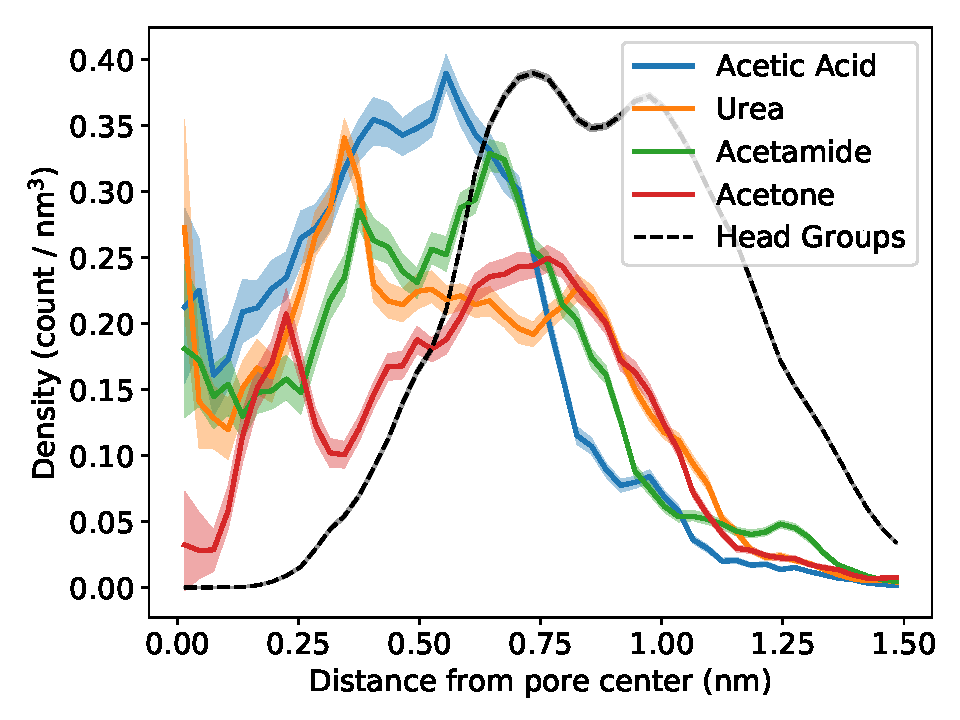
\includegraphics[width=\textwidth]{ketone_rdf.pdf}
  \caption{}\label{fig:ketones_rdf}
  \end{subfigure}
  \begin{subfigure}{0.45\textwidth}
  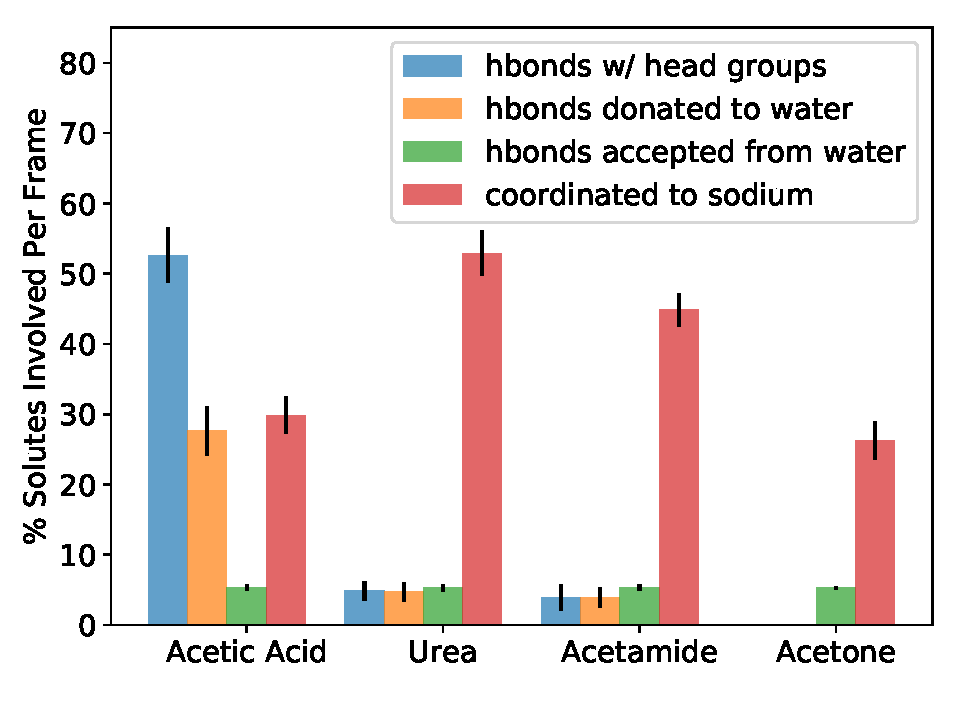
\includegraphics[width=\textwidth]{ketone_hbonds.pdf}
  \caption{}\label{fig:ketone_hbonds}
  \end{subfigure}
%  \begin{subfigure}{0.45\textwidth}
%  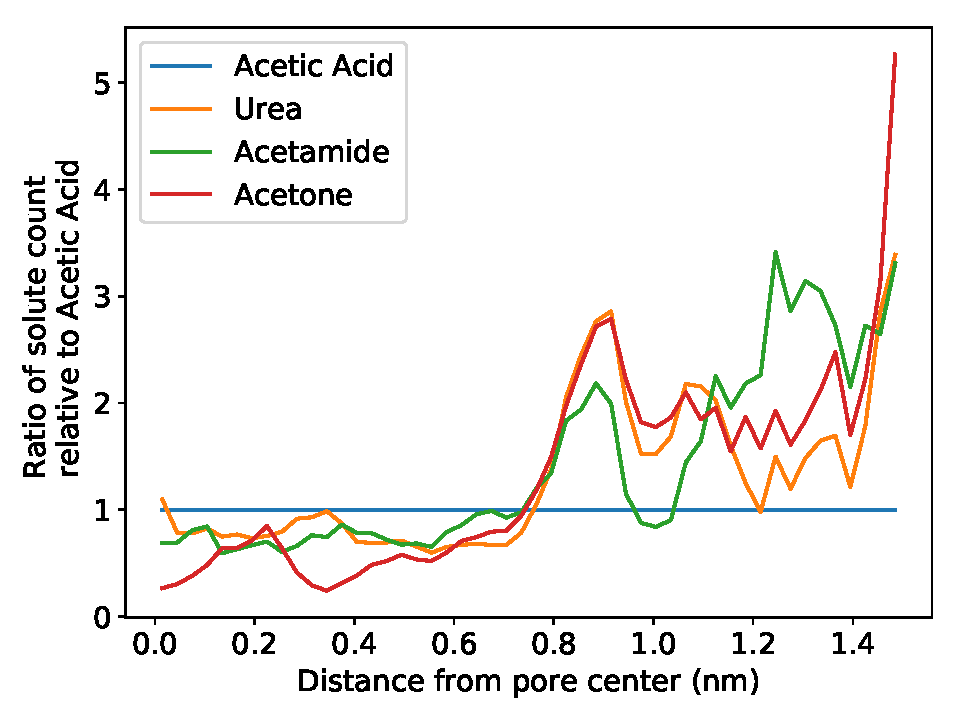
\includegraphics[width=\textwidth]{ketone_ratio.pdf}
%  \caption{}\label{fig:ketones_ratio}
%  \end{subfigure}
  \caption{(a) The radial density near the pore center (r = 0) decreases
  with decreasing solute MSD. (b) The amides hydrogen bond with water far
  less than acetic acid, however they tend to coordinate with sodium ions
  more frequently.}\label{fig:ketones}
  \end{figure}
  
  \subsection*{Transport of Thiols}
  
  We also studied the transport properties of sulfur analogs of glycerol, ethylene
  glycol and acetone.
%  Finally, we studied the transport properties of sulfur-containing compounds similar
%  to some of the solutes studied above.
  \begin{itemize}
    \item We replaced all but one oxygen atom of ethylene glycol and glycerol with sulfur atoms
    to create Dimercaptoethanol and 2,3-Dimercapto-1-propanol.
    \item We replaced the carbonyl carbon of acetone with sulfur in order to create DMSO. 
  	\item Sulfur is unable to hydrogen bond, however it is soluble in water  %BJC: maybe a reference to why sulfur can't hbond
 \end{itemize}
  	
%  	\item Comparisons of their RDFs are shown in Figure~\ref{fig:sulfur_analog_rdfs}.
%  \end{itemize}
  
  \begin{figure}
  \centering
  \begin{subfigure}{0.325\linewidth}
  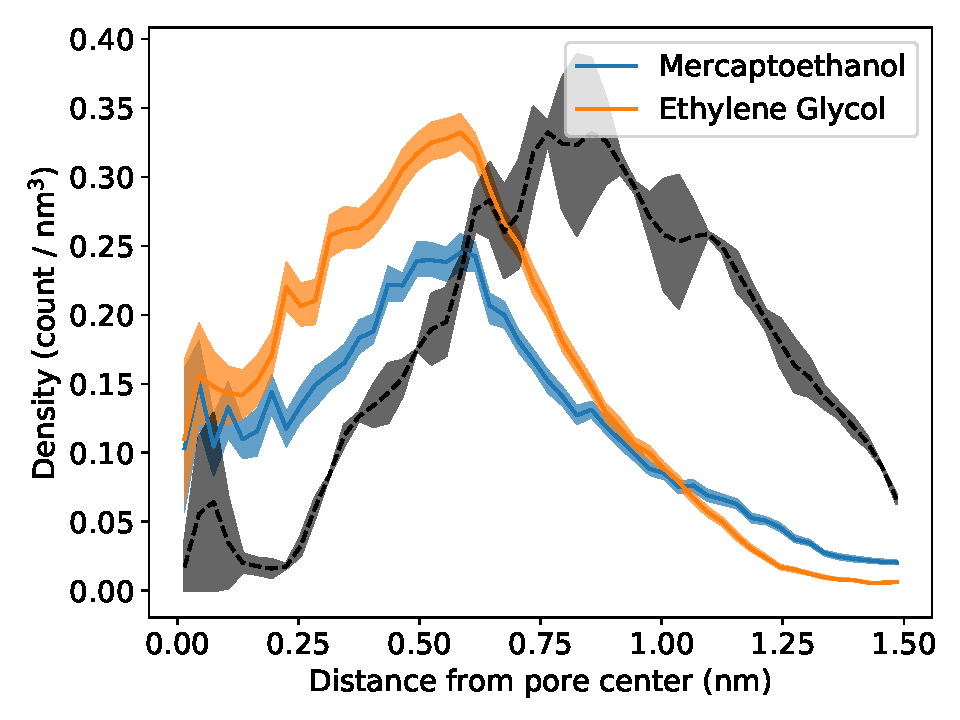
\includegraphics[width=\textwidth]{thiol_comparison_SOH.pdf}
  \caption{}\label{fig:SOH_GCL_comparison}
  \end{subfigure}
  \begin{subfigure}{0.325\linewidth}
  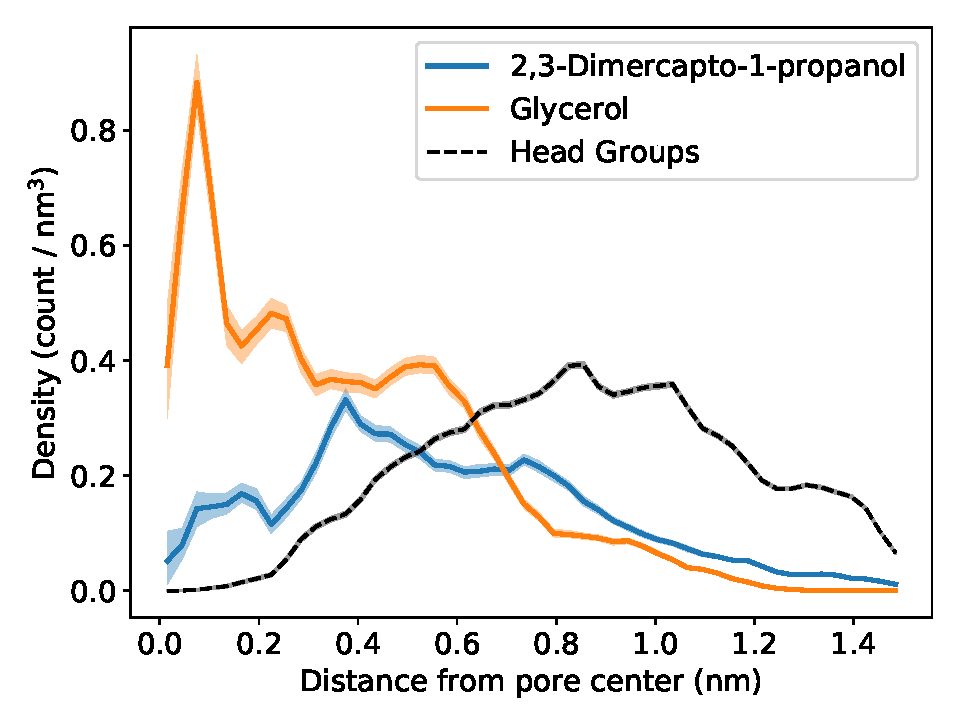
\includegraphics[width=\textwidth]{thiol_comparison_DMP.pdf}
  \caption{}\label{fig:DMP_GLY_comparison}
  \end{subfigure}
  \begin{subfigure}{0.325\linewidth}
  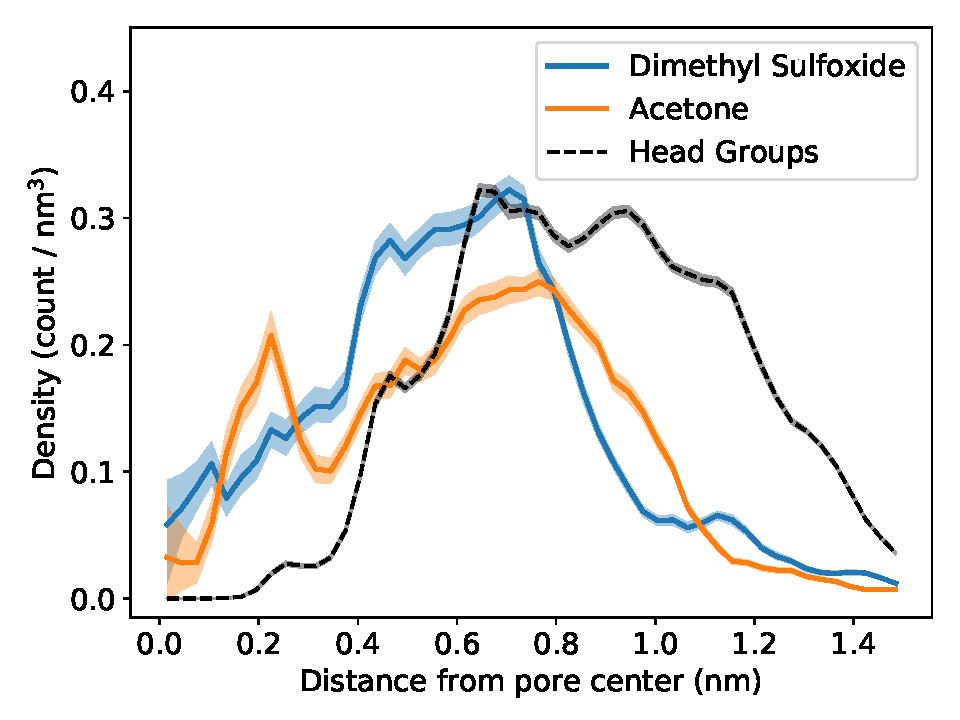
\includegraphics[width=\textwidth]{thiol_comparison_DMS.pdf}
  \caption{}\label{fig:DMP_GLY_comparison}
  \end{subfigure}
  \caption{(a) The RDF of mercaptoethanol is similar to ethylene glycol except 
  for its higher density in the tail region. (b) 2,3-Dimercapto-1-propanol is
  densest near the pore wall, unlike glycerol whose density is very high in the pore
  center. (c) Dimethylsulfoxide has a higher density than acetone close to the pore
  center which may in part explain its marginally larger MSD.}\label{fig:sulfur_analog_rdfs}
  \end{figure}
  
  \noindent Mercaptoethanol has a similar average MSD and RDF to ethylene glycol.
  \begin{itemize}
    \item There is a much larger uncertainty associated with mercaptoethanol's MSD.
    \item Some of this can be accounted for by the higher density of mercaptoethanol 
    molecules in the head group / tail region, where transport is inherently slower. 
    \item There are nearly 40 \% more mercaptoethanol molecules than ethylene 
    glycol molecules beyond 0.8 nm from the pore center. 
    \item Conversely, mercaptoethanol exhibits some of the highest single solute MSDs 
    (See Figure~\ref{fig:SOH_trace})  % Only methanol has greater (I think)
    \item It hydrogen bonds with head groups 6 times less frequently than ethylene glycol.
    \item This may lead to larger hops in the pore region.
%    \item When both hydroxyl groups of ethylene glycol are hydrogen bonded with the a
%    monomer head group simultaneously,
%    \item Less frequent hydrogen bonding and an affinity for the pore region may be
%    responsible for these hops.
  \end{itemize}
  
  %BJC: Could be a supporting figure
  \begin{figure}
  \centering
  \begin{subfigure}{0.45\textwidth}
  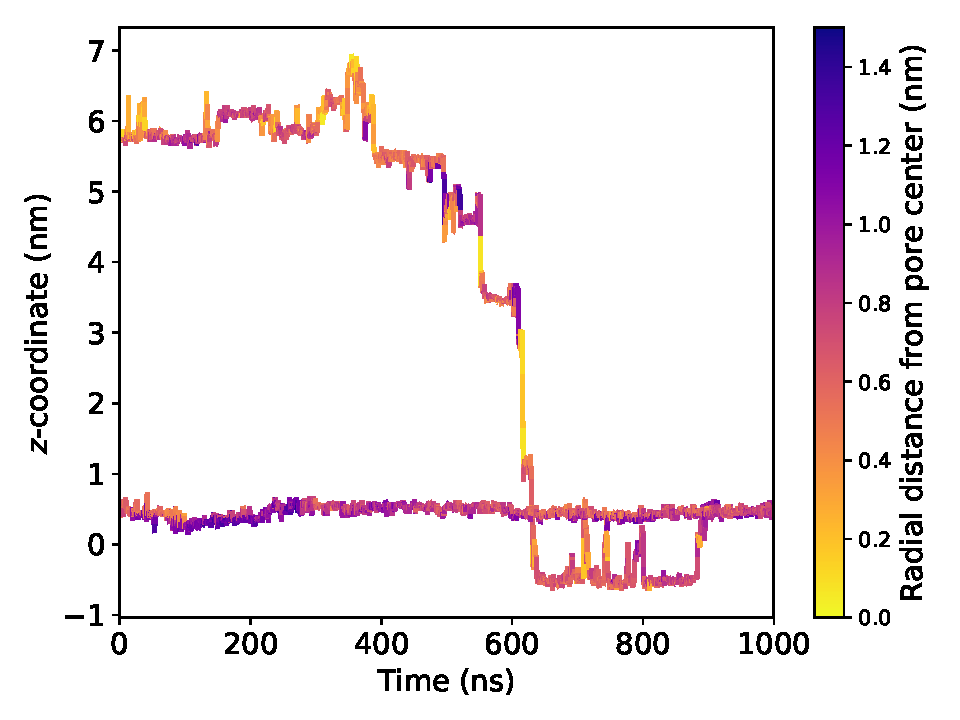
\includegraphics[width=\linewidth]{SOH_trace.pdf}
  \caption{}\label{fig:SOH_trace}
  \end{subfigure}
  \caption{Mercaptoethanol exhibits transport behavior ranging from frequent hopping
  to lengthy trapping. Large hops generally occur near the pore center while 
  long entrapments occur while tangled among the monomer tails.}
  \end{figure}
  
  % Potentially useful explanation
%  Ethylene glycol has a high chance of hydrogen bonding at least once with monomer head groups. 
%  An ethylene glycol molecule can hydrogen bond twice simultaneously.
%  When one of those hydrogen bond breaks, the molecule is still stabilized by another hydrogen bond
%  It can easily reform the second hydrogen bond in close proximity
  
  \noindent 2,3-Dimercapto-1-propanol exhibits slower transport than glycerol because it spends more time
  near monomer head groups. % BJC: should I give all the solutes nicknames (i.e. their residue names)?
  \begin{itemize}
    \item Glycerol frequently hydrogen bonds with more than one head group at a time (See Figure~\ref{fig:multi_hbonds}).
    % BJC: can probably quantify the following:
    \item It can also hydrogen bond with water molecules which increases its stability
    in the pore region.
    \item 2-3-Dimercapto-1-propanol preferentially hydrogen bonds with head groups 
    so it gravitates towards the head group region.
  \end{itemize} 
  
  \noindent DMSO has a comparable if not larger MSD than acetone even though it
  is a slightly larger molecule.
  \begin{itemize}
    \item The radial density of DMSO is higher than acetone close to the pore center.
  	\item The pyramidal structure of DMSO may force it to spend more time closer to
  	the pore center.
  	%BJC: quantify sodium coordination O group of DMSO
  \end{itemize}  
  
  \subsection*{Hydrogen bond acceptors}  % Need a better heading since all molecules in this study are acceptors

  %BJC: should probably at least mention acetone again in this section  
  The slowest set of molecules we studied can accept hydrogen bonds, but cannot donate
  them. 
  \begin{itemize}
  	\item Among this set are the two slowest solutes in our study: Tetrahydrofuran and Dimethyl Formamide.
  	\item The MSDs of ethyl acetate, propylene carbonate and acetone are only marginally larger.
  	% EAC and PCB are both larger molecules. Acetone is small. %BJC: not sure how far I should dive into this point
  \end{itemize}  
  
%  The radial density functions highlight the solutes' preference for the 
%  head group region.
%  \begin{itemize}
%  	\item There are small peaks in the radial density greater than 1 nm 
%  	from the pore center.
%  	\item The solutes become trapped in these regions where each step is
%  	highly anti-correlated to its previous step, leading to very low MSDs.
%  	\item The large size and nonplanar shapes of ethyl acetate and propylene 
%  	carbonate may destabilize entrapment in the tail region more quickly, leading
%  	to slightly faster transport. 
%  	% BJC:  Ethyl acetate spends all of its time in a linear or near-linear conformation.
%  \end{itemize}
  
  \noindent The radial density of solutes near the pore center in this set is surprisingly high
  as shown in Figure~\ref{fig:nondonors_rdf}.
  \begin{itemize}
    \item Propylene carbonate and ethyl acetate are among the largest solutes
    in this study. Their size prevents them from easily entering the tail 
    region and generally gives faster transport properties since they spend
    more time in the pore region. 
    \item However, this is not a hard rule. When a solute does overcome the 
    barrier of entry beyond the head group region, it can become trapped. All
    solutes in this set show a peak $\geq$ 1 nm from the pore center which is
    likely caused by solutes that get trapped in the tail region for a significant
    amount of time.
	\item The peak density of THF is considerably offset from the pore center.
	\item Observations of single THF trajectories have revealed that it does not make
	large hops while in the pore center.
	\item THF becomes nearly immobilized while associated with sodium ions (See 
	Figure~\ref{fig:thf_sodium_coordination}).
	\item DMF experiences a similar effect, but to a lesser extent. Its density is 
	higher than THF near the head groups. The planar shape of DMF causes it to 
	become stuck between head groups. Excursions into the pore region do not
	necessarily result in large hops.
  \end{itemize}
  
  \noindent Carbonyl groups continue to show high degrees of association with sodium ions. 
  \begin{itemize}
    \item The number of sodium ions coordinated to the carbonyl group of 
    propylene carbonate, dimethyl formamide, ethyl acetate are consistent with 
    that shown by acetone, all between 6 and 7 per frame (See 
    figure~\ref{fig:nondonors_hbonds})
    \item The carbonyl group of the amides studied in the previous section
    associate with sodium nearly twice as frequently as compounds that don't
    contain nitrogen (see figure~\ref{fig:ketone_hbonds}).
    \item In all cases, other polar groups on carbonyl-containing compounds
    associate with sodium in negligible amounts.
  \end{itemize}
 
  \begin{figure}
  \centering
  \begin{subfigure}{0.45\textwidth}
  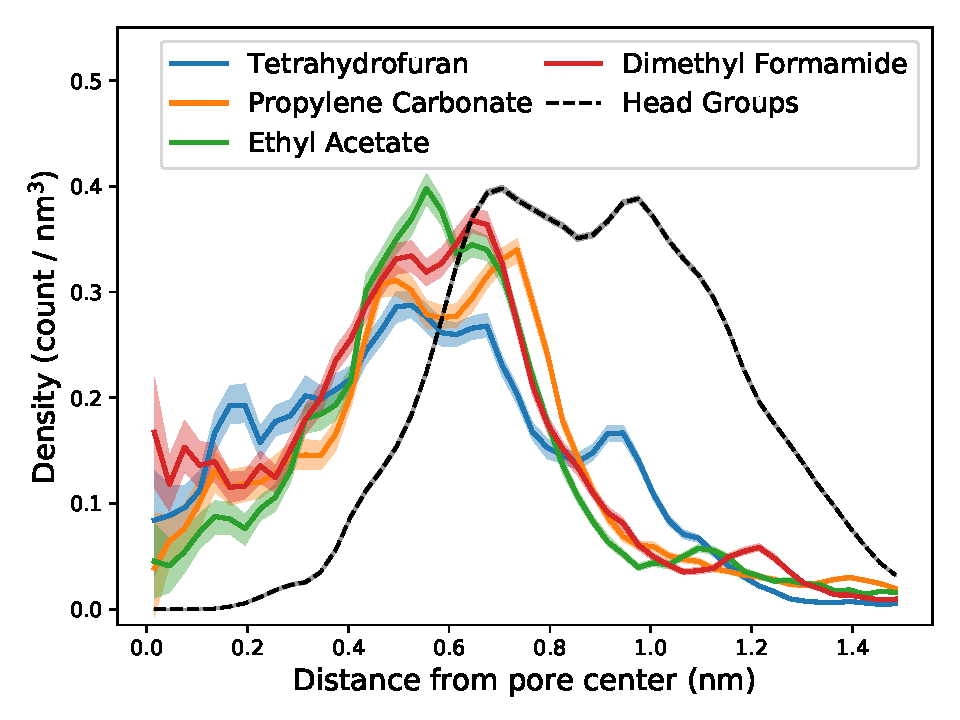
\includegraphics[width=\textwidth]{nondonors_rdf.pdf}
  \caption{}\label{fig:nondonors_rdf}
  \end{subfigure}
  \begin{subfigure}{0.45\textwidth}
  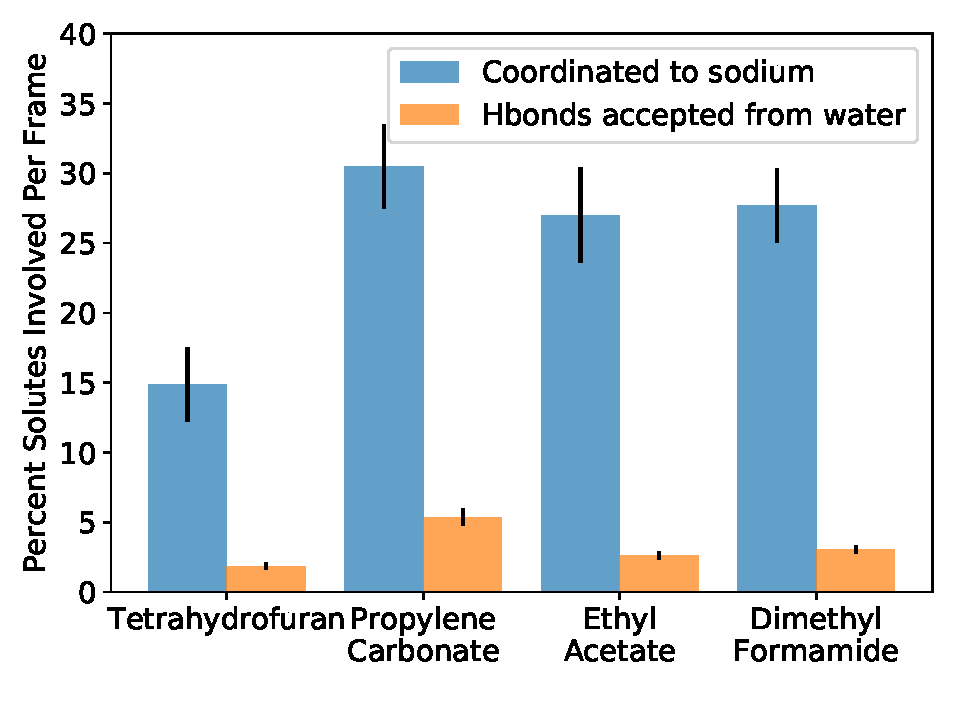
\includegraphics[width=\textwidth]{nondonor_hbonds.pdf}
  \caption{}\label{fig:nondonors_hbonds}
  \end{subfigure}
  \end{figure}
  
  \begin{figure}
  \centering
  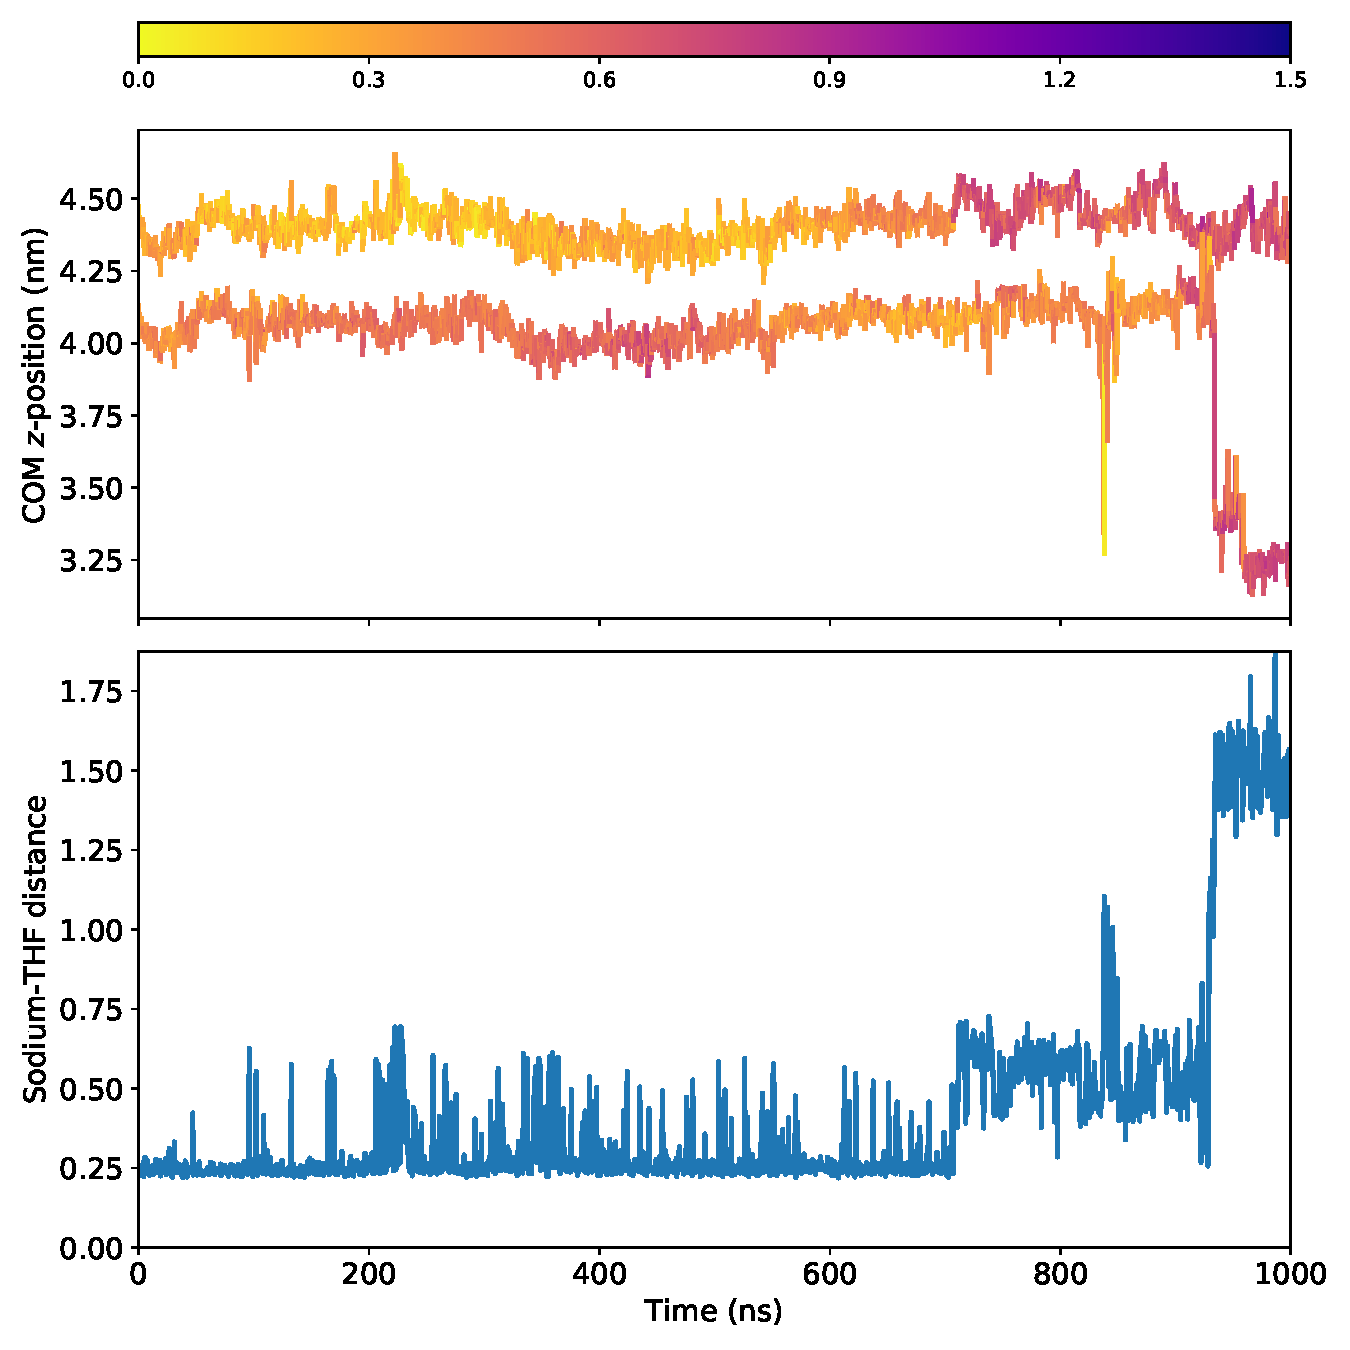
\includegraphics[width=0.5\textwidth]{thf_sodium_coordination.pdf}
  %BJC: figure was hard to make exactly how I wanted it so I stopped until we decide the best way to illustrate this point
  %BJC: Should I do two colorbars (one for sodium, one for THF)
  %BJC: Should Sodium-THF distance be between THF COM and sodium in order to be consistent with above figure? 
  \caption{Coordination of THF with sodium ions may help stabilize it inside the
  pore region. For the first 700 ns of the trajectories shown, the center of mass
  of THF (top line in top figure) and a sodium ion (bottom line in top figure) move
  in tandem. The distance between the oxygen atom of THF and the sodium ion has only
  occasional fluctuations away from a relatively stable separation of ca. 0.25 nm. 
  After 700 ns, THF separates from the sodium ion and moves closer to the head group
  region.}\label{fig:thf_sodium_coordination}
  \end{figure}
  
  % THF shows highly anticorrelated hops
  
%  The majority of THF trajectories are spent near or beyond the head groups. Some
%  trajectories spend all of their time near the pore center but with very little movement. 
%  High densities in head group / tail region is a consequence of trajectories where THF
%  gets trapped there. Ring structure of THF makes it miscible with water (has dipole). Bulky alkyl
%  substituents are kept from interfering with oxygen's electron pairs. THF does not
%  make large hops in the pore center for some reason.
%  Water does not get close to THF when it's in the pore center
%  THF appears to prefer to associate with sodium 
%  THF is stabilized by sodium or by a hydrogen bond with water leaving oily groups alone which
%  don't want to move through the water. The effective size of THF increases and prevents it
%  from moving.
%  
%  DMF shows similar characteristics, however spends a large proportion of its time trapped 
%  between head groups.
  
  %All have comparable densities near pore center except acetone which is lower

  \subsection{Design Considerations}

  Based on our observations of the complex interactions between various polar solutes
  and the membrane's liquid crystal monomers, we can speculate on design criteria for 
  the next generation of liquid crystal monomers to be used for LLC membrane
  synthesis.
  \begin{itemize}
    \item Unfortunately, we cannot comment on the stability of the H\textsubscript{II}
    phase if major changes are made to the monomers.
    \item Therefore, our most feasible design suggestions are those which can be made
    as a post-processing step to the cross-linked membrane created using Na-GA3C11.
  \end{itemize}
  
  The transport properties of solutes are a strong function of the 3 trapping
  mechanisms discussed above. Therefore, it is most logical to design monomers with 
  them in mind. 
  
  Since solutes move slowly well entangled among the monomer tails, one can try to
  design monomers that better control the partition of solutes between the pore and
  tail region.
  \begin{itemize}
    \item The head groups of Na-GA3C11 are planar which leaves a fair amount of space
    between adjacent head groups and it makes it easier for solutes to slip between and
    past them.
    \item Bulkier substituents, which do not impede stacking of monomers into columns,
    might slow the rate at which solutes partition into the tails.
    \item Additionally, one can include crosslinkable groups near the head groups in
    order to fill free volume and effectively create a wall.
    \item Finally, removal of the ether linkages between the head groups and the monomer
    tails will decrease the stability of polar molecules in the head group region.
    \item Overall, controlling the solute partition might not be the most important 
    consideration to optimize because once enough solutes flow through, the membrane tail
    region will become saturated with solute molecules and greatly reduce the rate of partition.
  \end{itemize}
  
  Alternatively, one can focus on designing head groups with varying hydrogen 
  bonding capabilites.
  \begin{itemize}
    \item Na-GA3C11 has a carboxylate group which readily accepts hydrogen bonds
    \item One can increase the number of hydrogen bonding sites on the head groups
    in order to trap more solutes, or decrease the number of hydrogen bond sites
    to trap less.
  \end{itemize}
  
  Finally, one can attempt to control the degree to which solutes coordinate 
  with counterions.
  \begin{itemize}
    \item We have observed a significant amount of sodium association with 
    negatively charge solute constituents.
    \item Changing the size and valence of the counter ion may offer some
    interesting behavior. 
    \item For example, a counter ion with a charge of +2 may attract more solute
    molecules and bind them more tightly, but there will only be half as many
    counterions in the system which may reduce its overall influence.
    \item Additionally, the size of the counterion will affect the mobility
    of any complex formed. 
    \item Sodium appears to do a good job of immobilizing complexes formed between
    it and solutes. 
    \item However, a Lithium ion might be more prone to go along for the ride.
    \item Hydrogen would likely spend the majority of its time bound to the 
    carboxylate head group or as part of a hydronium ion hence interfering with 
    solute transport infrequently.
  \end{itemize}
  
%  There are two types of separations for which this membrane may have some use.
%  \begin{enumerate}
%    \item In a purification process, one may only desire water to pass. In this 
%    case, water should have much faster dynamics than any other dissolved species.~\label{sep:purification}
%    \item For a separate application, one may desire to selectively separate a 
%    dissolved species from a complex stream.~\label{sep:selective}
%  \end{enumerate}
  
  The MSD of solutes may be much larger in more concentrated solutions because there
  will be less available trapping sites for them to occupy.
  \begin{itemize}
    \item We purposely studied the behavior of the solutes in dilute conditions.
    \item The difference in size between water and the fastest solute, methanol, is not
    enough to explain the order of magnitude difference in their average MSDs.
    \item The sheer number of water molecules prevents the majority of them from 
    becoming trapped for long periods of time.
    \item A similar effect may increase solute MSDs in more concentrated solutions.
  \end{itemize}
  
  As a final consideration, water content affects pore size and strongly influences
  the MSDs of solutes, water and counterions.
  \begin{itemize}
    \item The MSD of these components is about 2 orders of magnitude larger in the 
    10 wt \% system than the 5 wt \% system.
    \item The 5 wt \% system is much less feasible as a separations membrane on the basis
    of water permeability alone.
    \item Typically, the total water content used to create the H\textsubscript{II} phase
    is reported, but the amount of water that resides in the pores, tails and in between
    hexagonal mesophases is less clear.
    \item Experiments, such as those by Jenkins et al.~\cite{jenkins_identification_2012}, 
    may help elucidate the water composition in each region.
    \item The results would be extremely useful for determining the viability of a given
    LLC membrane system. 
  \end{itemize}

  \section{Conclusion}

  We have examined the transport characteristics of a series of small polar
  molecules in our model of the H\textsubscript{II} phase formed by the liquid 
  crystal monomer Na-GA3C11.

  We learned that the MSD of solutes, water and counter ions are highly dependent 
  on LLC membrane water content.
  \begin{itemize}
    \item As more water is added to the system, the pores become less crowded
    with monomer components and the MSD of water, sodium and solutes increase.
    \item The amount of water in the pores deserves special attention when 
    screening new monomers.
  \end{itemize}

  We learned that solutes undergo anomalous diffusion which can be described 
  as a subordinated fractional brownian motion process. 
  \begin{itemize}
    \item In general, solutes hop intermittently between periods of entrapment
    \item These hops are anti-correlated to their previous hops
  \end{itemize}
  
  We observed three mechanisms of solute entrapment.
  \begin{itemize}
    \item A solute can become stuck in the tail region. 
    \item A solute can hydrogen bond with monomers
    \item A solute can associate with a bound counterion
  \end{itemize}
  
  Based on these trapping mechanisms, we have suggested modifications that
  can be made to monomers in order to mitigate or enhance their effect on
  solute MSDs.
 
  \section*{Supporting Information}

  Detailed explanations and expansions upon the results and procedures mentioned in
  the main text are described in the Supporting Information. This information is
  available free of charge via the Internet at http://pubs.acs.org.

  \section*{Acknowledgements}

  Molecular simulations were performed using the Extreme Science and
  Engineering Discovery Environment (XSEDE), which is supported by National
  Science Foundation grant number ACI-1548562. Specifically, it used the Bridges
  system, which is supported by NSF award number ACI-1445606, at the Pittsburgh
  Supercomputing Center (PSC). This work also utilized the RMACC Summit supercomputer,
  which is supported by the National Science Foundation (awards ACI-1532235 and
  ACI-1532236), the University of Colorado Boulder, and Colorado State
  University. The Summit supercomputer is a joint effort of the University of
  Colorado Boulder and Colorado State University.

  \clearpage

  \bibliographystyle{ieeetr}
  \bibliography{transport}

  \newpage

  \section*{TOC Graphic}

\end{document}
